\documentclass[dvipdfmx,aspectratio=169,11pt]{beamer}
\usetheme{Madrid}
\usecolortheme{seahorse}
\setbeamertemplate{navigation symbols}{}
\setbeamertemplate{headline}{}
\setbeamertemplate{footline}[frame number]
\setbeamertemplate{frametitle continuation}{}
\setbeamertemplate{frametitle}{\nointerlineskip\begin{beamercolorbox}[wd=\paperwidth,sep=0.45ex,leftskip=7.5mm,rightskip=7.5mm]{frametitle}\usebeamerfont{frametitle}\insertframetitle\end{beamercolorbox}}
\setbeamerfont{frametitle}{size=\large}
\setbeamerfont{normal text}{size=\normalsize}
\setbeamersize{text margin left=8mm,text margin right=8mm}
\setbeamercolor{keyphrase}{bg=blue!8,fg=black!85}
\setbeameroption{hide notes}
\usepackage{pgfpages}
\pgfpagesuselayout{resize to}[a4paper,landscape]
\usepackage[T1]{fontenc}
\usepackage{tabularx}
\usepackage{array}
\usepackage{booktabs}
\usepackage{listings}
\usepackage{hyperref}
\usepackage{fancyvrb}
\usepackage{bxdpx-beamer}
\usepackage{pxjahyper}
\renewcommand{\kanjifamilydefault}{\gtdefault}
\setbeamertemplate{itemize items}[circle]
\setbeamertemplate{enumerate items}[default]
\institute{岩手県立大学}
\lstdefinelanguage{mizar}{morekeywords={definition,end,struct,field,property,inherit,extends,where,from,let,be,being,mode,theorem,proof,thus,hence,by,registration,cluster,coherence,reduce,reducibility,import,for,holds,st,is,func,pred,attribute,algorithm,terminating,requires,ensures,do,while,invariant,decreasing,return,var,const,if,scheme,provided,environ,vocabularies,notations,constructors,registrations,theorems,begin,qua,reconsider,consider,such,that,not,or,and,implies,per,cases,set,thesis},sensitive=true,morecomment=[l]{::}}
\lstdefinelanguage{toml}{morecomment=[l]{\#},morestring=[b]"}
\lstset{basicstyle=\ttfamily\small,keywordstyle=\color{blue!50!black}\bfseries,commentstyle=\color{green!35!black}\itshape,stringstyle=\color{violet!70!black},showstringspaces=false,columns=fullflexible,keepspaces=true,backgroundcolor=\color{black!4},frame=single,rulecolor=\color{black!20},framesep=0.7mm,framerule=0.3pt,xleftmargin=1mm,xrightmargin=1mm,aboveskip=0.6mm,belowskip=0.8mm}
\newcommand{\statusbadge}[2]{\colorbox{#1}{\textcolor{white}{\strut\scriptsize\sffamily\bfseries #2}}}
\newcommand{\badgeMML}{\statusbadge{blue!45!black}{exact MML excerpt}}
\newcommand{\badgeSpec}{\statusbadge{green!35!black}{specification example}}
\newcommand{\badgeSketch}{\statusbadge{orange!75!black}{sketch}}
\newcommand{\deepdivetag}{\hfill\colorbox{black!15}{\textcolor{black!65}{\strut\scriptsize\sffamily deep dive}}}
\pdfstringdefDisableCommands{\def\translate#1{#1}}
\title{Mizar Evo の設計指針について}
\subtitle{自動証明・数学的記述・検証可能な計算の再接続}
\author{中正 和久}
\date{TPP 2026、理化学研究所 AIP 東京オフィス、2026年11月16--17日}

\begin{document}
\begin{frame}
\titlepage
\note{
\smallskip
\textbf{Read aloud:}
\begin{itemize}
\setlength{\itemsep}{1pt}
\setlength{\parsep}{0pt}
\setlength{\parskip}{0pt}
\item \textcolor{blue!55!black}{\textbf{Mizar は証明検査系です。一階の集合論の上に、人間が読める数学の言葉で書かれた50年分のライブラリを持っています。}}
\item \textcolor{blue!55!black}{\textbf{Mizar Evolution、略して Mizar Evo は、その言語と道具を設計し直すプロジェクトです。現行 Mizar の課題を整理し、新仕様でどのように対応するかを説明します。}}
\item 話す内容にはすべて、事実・研究仮説・将来構想のラベルを付けます。
\end{itemize}
}
\end{frame}

\section{Part 0. Introduction}
\begin{frame}[fragile,t]{0.3 - 現行 Mizar の課題と6つの設計指針}
\begin{footnotesize}
\setlength{\tabcolsep}{3pt}
\renewcommand{\arraystretch}{1.15}
\begin{tabularx}{\textwidth}{>{\raggedright\arraybackslash}X>{\raggedright\arraybackslash}X}
\toprule
\textbf{現行 Mizar から取り組む課題} & \textbf{新仕様の設計指針} \\
\midrule
\textcolor{blue!55!black}{\textbf{§1 基盤:}} 論理・MML の継承と処理系の刷新 & 一階論理・集合論を維持し、kernel を小さく保つ \\
\textcolor{blue!55!black}{\textbf{§2 記述:}} 暗黙の型・登録・演算選択の追跡 & 数学的な抽象化を継承し、暗黙の選択を明示 \\
\textcolor{blue!55!black}{\textbf{§3 汎用化:}} 定義・定理・scheme の個別機構 & template で共通化の仕組みを統一 \\
\textcolor{blue!55!black}{\textbf{§4 計算:}} 証明と実行可能な手続きの接続 & algorithm の契約・不変条件・停止性を検査 \\
\textcolor{blue!55!black}{\textbf{§5 開発基盤:}} 依存管理・配布・差分検証・IDE & module・namespace・package・差分ビルド・LSP \\
\textcolor{blue!55!black}{\textbf{§6 検査・自動化:}} 外部探索と検査根拠の接続 & ATP を活用し、evidence のインスタンス化と SAT 検査 \\
\bottomrule
\end{tabularx}
\end{footnotesize}

\note{
Optional detail (see slide).

\smallskip
\textbf{Optional notes and sources:}
\begin{itemize}
\setlength{\itemsep}{1pt}
\setlength{\parsep}{0pt}
\setlength{\parskip}{0pt}
\item 課題と設計指針を同じ行に対応させる。以下の §1–§6 が各行に対応。一階の基盤と可読な記述は、継承すべき強み。
\item 新仕様と実装済みの範囲は、末尾の「仕様と実装の状況」で区別する。
\item Source: 仕様 01, 18, 20, 21, 23; Bia\l{}ystok 資料の課題別ストーリー。
\end{itemize}
}
\end{frame}

\section{Part 1. Logical Foundation}
\begin{frame}[fragile,t]{1.1 - 基盤の継承: 論理は保ち、処理系を再整備}
\begin{center}
\begin{beamercolorbox}[rounded=true,sep=2.5mm,wd=0.9\textwidth]{keyphrase}
\centering\itshape \textcolor{blue!55!black}{\textbf{数学的記述の層を継承し、}}\\ \textcolor{blue!55!black}{\textbf{処理系と開発基盤を再構築する。}}
\end{beamercolorbox}
\end{center}
\begin{itemize}
\setlength{\itemsep}{1pt}
\setlength{\parsep}{0pt}
\setlength{\parskip}{0pt}
\item \textcolor{blue!55!black}{\textbf{一階論理と Tarski-Grothendieck 集合論を基盤として維持。}}
\item soft type、mode、attribute、registration、structure、宣言的証明を継承。
\item \textcolor{blue!55!black}{\textbf{証明探索と検査を分離し、受理を小規模な kernel に集約。詳細は §6。}}
\end{itemize}
\note{
\smallskip
\textbf{Read aloud:}
\begin{itemize}
\setlength{\itemsep}{1pt}
\setlength{\parsep}{0pt}
\setlength{\parskip}{0pt}
\item \textcolor{blue!55!black}{\textbf{数学的記述の層を継承し、}} \textcolor{blue!55!black}{\textbf{処理系と開発基盤を再構築する。}}
\item \textcolor{blue!55!black}{\textbf{一階論理と Tarski-Grothendieck 集合論を基盤として維持。}}
\item soft type、mode、attribute、registration、structure、宣言的証明を継承。
\item \textcolor{blue!55!black}{\textbf{証明探索と検査を分離し、受理を小規模な kernel に集約。詳細は §6。}}
\end{itemize}
\smallskip
\textbf{Optional notes and sources:}
\begin{itemize}
\setlength{\itemsep}{1pt}
\setlength{\parsep}{0pt}
\setlength{\parskip}{0pt}
\item 数学的な記述と証明支援に必要な機能は、一階の基盤の上にも構成できる。「仕組みが近い」はこれらの構成を指し、論理体系や表現方法の同一性を意味しない。
\item 成功率や再構成の失敗率から一階の性能優位性を主張しない。設計の効果は、記述の利便性・自動証明・証明検査の観点で評価する。
\end{itemize}
}
\end{frame}

\begin{frame}[fragile,t]{1.2 - 現行 Mizar: 集合論的な関数}
\smallskip
\textbf{関数適用は定義された集合論的関係}~\badgeMML
\begin{lstlisting}[language={mizar},basicstyle=\ttfamily\small]
  func f.x -> set means
  :Def2:
  [x,it] in f if x in dom f otherwise it = {};
\end{lstlisting}
\smallskip
\textbf{型付き関数は部分関数の上の soft type}~\badgeMML
\begin{lstlisting}[language={mizar},basicstyle=\ttfamily\small]
definition
  let X,Y;
  mode Function of X,Y is quasi_total PartFunc of X,Y;
end;
\end{lstlisting}
\begin{itemize}
\setlength{\itemsep}{1pt}
\setlength{\parsep}{0pt}
\setlength{\parskip}{0pt}
\item \textcolor{blue!55!black}{\textbf{関数は対の集合として表される一階の対象。関数適用は集合論上で定義する。}}
\item \textcolor{blue!55!black}{\textbf{関数の扱いに、基盤論理の高階化は不要。}}
\item 記述上の課題: 定義域・グラフ・関数性・所属関係を直接記述すると煩雑。
\end{itemize}
\note{
\smallskip
\textbf{Read aloud:}
\begin{itemize}
\setlength{\itemsep}{1pt}
\setlength{\parsep}{0pt}
\setlength{\parskip}{0pt}
\item 関数適用は定義された集合論的関係.
\item 型付き関数は部分関数の上の soft type.
\item \textcolor{blue!55!black}{\textbf{関数は対の集合として表される一階の対象。関数適用は集合論上で定義する。}}
\item \textcolor{blue!55!black}{\textbf{関数の扱いに、基盤論理の高階化は不要。}}
\item 記述上の課題: 定義域・グラフ・関数性・所属関係を直接記述すると煩雑。
\end{itemize}
\smallskip
\textbf{Optional notes and sources:}
\begin{itemize}
\setlength{\itemsep}{1pt}
\setlength{\parsep}{0pt}
\setlength{\parskip}{0pt}
\item Source（2026年10月7日確認）: \url{https://mizar.uwb.edu.pl/version/current/mml/funct\_1.miz}（138-140 行、\texttt{FUNCT\_1:def 2}）、\url{https://mizar.uwb.edu.pl/version/current/mml/funct\_2.miz}（87-90 行）。GPL-3.0-or-later / CC-BY-SA-3.0-or-later。
\item \texttt{quasi\_total}（FUNCT\_2 の 36-44 行）は、Y が空でなければ定義域が X 全体であることを言う。
\end{itemize}
}
\end{frame}

\section{Part 2. Readable Mathematics}
\begin{frame}[fragile,t]{2.1 - 記述の課題: 可読性と抽象化を継承・拡張}
\smallskip
\textbf{ソース上の関数表現}~\badgeSketch~{\footnotesize(現行 Mizar と Mizar Evo で有効)}
\begin{lstlisting}[language={mizar},basicstyle=\ttfamily\small]
let X, Y be set;
let f be Function of X, Y;
let x be Element of X;
...  f.x  ...
\end{lstlisting}
\begin{itemize}
\setlength{\itemsep}{1pt}
\setlength{\parsep}{0pt}
\setlength{\parskip}{0pt}
\item \textcolor{blue!55!black}{\textbf{集合論的な関数を \texttt{Function of X,Y} と \texttt{f.x} で記述し、対や定義域の詳細を抽象化する。}}
\item \textcolor{blue!55!black}{\textbf{soft type、mode、attribute、registration、scheme、宣言的証明は、単なる記法の簡略化を超え、一階の集合論を可読な数学的記述へ結び付ける言語機構。}}
\item \textcolor{blue!55!black}{\textbf{新仕様: 数学的な記述を継承・拡張し、型・登録・オーバーロードの暗黙の選択を明示・追跡可能にする。}}
\end{itemize}
\note{
\smallskip
\textbf{Read aloud:}
\begin{itemize}
\setlength{\itemsep}{1pt}
\setlength{\parsep}{0pt}
\setlength{\parskip}{0pt}
\item ソース上の関数表現.
\item \textcolor{blue!55!black}{\textbf{集合論的な関数を \texttt{Function of X,Y} と \texttt{f.x} で記述し、対や定義域の詳細を抽象化する。}}
\item \textcolor{blue!55!black}{\textbf{soft type、mode、attribute、registration、scheme、宣言的証明は、単なる記法の簡略化を超え、一階の集合論を可読な数学的記述へ結び付ける言語機構。}}
\item \textcolor{blue!55!black}{\textbf{新仕様: 数学的な記述を継承・拡張し、型・登録・オーバーロードの暗黙の選択を明示・追跡可能にする。}}
\end{itemize}
}
\end{frame}

\begin{frame}[fragile,t]{2.2 - Registration: 自動的な連鎖に名前を付ける}
\smallskip
\textbf{ラベルを持つ自動適用規則}~\badgeSpec
\begin{lstlisting}[language={mizar},basicstyle=\ttfamily\small]
registration
  cluster EmptyImpliesFinite: empty -> finite for set;
  coherence proof ... end;
  cluster FiniteImpliesCountable: finite -> countable for set;
  coherence proof ... end;
end;
\end{lstlisting}
\begin{footnotesize}
\setlength{\tabcolsep}{3pt}
\renewcommand{\arraystretch}{1.15}
\begin{tabularx}{\textwidth}{>{\raggedright\arraybackslash}X>{\raggedright\arraybackslash}X>{\raggedright\arraybackslash}X}
\toprule
\textbf{出発点} & \textbf{自動的に得られる事実} & \textbf{記録する規則} \\
\midrule
S is empty & S is finite & EmptyImpliesFinite \\
S is finite & S is countable & FiniteImpliesCountable \\
\bottomrule
\end{tabularx}
\end{footnotesize}

\begin{itemize}
\setlength{\itemsep}{1pt}
\setlength{\parsep}{0pt}
\setlength{\parskip}{0pt}
\item \textcolor{blue!55!black}{\textbf{連鎖的な自動適用を保ち、各登録項目のラベルを必須にして、適用経路を記録する。}}
\item 証明がどの規則に依存するかを説明できる。自動適用のために \texttt{by} で明示引用する必要はない。
\end{itemize}
\note{
\smallskip
\textbf{Read aloud:}
\begin{itemize}
\setlength{\itemsep}{1pt}
\setlength{\parsep}{0pt}
\setlength{\parskip}{0pt}
\item ラベルを持つ自動適用規則.
\item \textcolor{blue!55!black}{\textbf{連鎖的な自動適用を保ち、各登録項目のラベルを必須にして、適用経路を記録する。}}
\item 証明がどの規則に依存するかを説明できる。自動適用のために \texttt{by} で明示引用する必要はない。
\end{itemize}
\smallskip
\textbf{Optional notes and sources:}
\begin{itemize}
\setlength{\itemsep}{1pt}
\setlength{\parsep}{0pt}
\setlength{\parskip}{0pt}
\item Source: \texttt{doc/spec/en/17.clusters\_and\_registrations.md} §17.2, 17.7; \texttt{23.package\_management\_and\_build\_system.md} §23.7.7。表は empty set S の説明用トレース。属性の解決は ATP 探索より前に行う。
\end{itemize}
}
\end{frame}

\begin{frame}[fragile,t]{2.3 - 構造: 格納する field と導出する property}
\smallskip
\textbf{データと標準的な値を分ける}~\badgeSpec
\begin{lstlisting}[language={mizar},basicstyle=\ttfamily\small]
definition
  struct AddLoopStr where
    field carrier -> set;
    field add -> BinOp of carrier;
    property zero -> Element of carrier;
  end;
end;
\end{lstlisting}
\begin{itemize}
\setlength{\itemsep}{1pt}
\setlength{\parsep}{0pt}
\setlength{\parskip}{0pt}
\item \textcolor{blue!55!black}{\textbf{field は格納するデータで、構成子の引数。property の一意な値は、別の実装で与える。}}
\item \texttt{zero} の宣言は型を与える。\texttt{means} 実装は存在・一意性を証明し、\texttt{equals} 実装は値を表す項を与える。
\end{itemize}
\note{
\smallskip
\textbf{Read aloud:}
\begin{itemize}
\setlength{\itemsep}{1pt}
\setlength{\parsep}{0pt}
\setlength{\parskip}{0pt}
\item データと標準的な値を分ける.
\item \textcolor{blue!55!black}{\textbf{field は格納するデータで、構成子の引数。property の一意な値は、別の実装で与える。}}
\item \texttt{zero} の宣言は型を与える。\texttt{means} 実装は存在・一意性を証明し、\texttt{equals} 実装は値を表す項を与える。
\end{itemize}
\smallskip
\textbf{Optional notes and sources:}
\begin{itemize}
\setlength{\itemsep}{1pt}
\setlength{\parsep}{0pt}
\setlength{\parskip}{0pt}
\item Source: \texttt{doc/spec/en/05.structures.md} §5.2; \texttt{07.modes.md} §7.4.1, 7.8.2; \texttt{sample\_codes.md}, AddLoopStr。property の実装が重なる場合は coherence が必要。
\end{itemize}
}
\end{frame}

\begin{frame}[fragile,t]{2.3a - 継承関係を後から宣言する}
\smallskip
\textbf{AddLoopStr の宣言後に、親への対応付けを追加}~\badgeSpec
\begin{lstlisting}[language={mizar},basicstyle=\ttfamily\small]
definition
  inherit AddLoopStr extends LoopStr where
    field carrier from carrier;
    field add from binop;
    property zero from unit;
  end;
end;
\end{lstlisting}
\begin{itemize}
\setlength{\itemsep}{1pt}
\setlength{\parsep}{0pt}
\setlength{\parskip}{0pt}
\item \textcolor{blue!55!black}{\textbf{構造の宣言と継承関係を分離。型を定義した後で Rust の trait を実装する構成に近い。}}
\item \texttt{from} で親の役割をリネーム: \texttt{binop} を \texttt{add}、\texttt{unit} を \texttt{zero} に対応付ける。
\item 親ごとに一つの宣言。同じメンバー型なら証明不要、型を狭める場合は \texttt{coherence} を証明する。
\end{itemize}
\note{
\smallskip
\textbf{Read aloud:}
\begin{itemize}
\setlength{\itemsep}{1pt}
\setlength{\parsep}{0pt}
\setlength{\parskip}{0pt}
\item AddLoopStr の宣言後に、親への対応付けを追加.
\item \textcolor{blue!55!black}{\textbf{構造の宣言と継承関係を分離。型を定義した後で Rust の trait を実装する構成に近い。}}
\item \texttt{from} で親の役割をリネーム: \texttt{binop} を \texttt{add}、\texttt{unit} を \texttt{zero} に対応付ける。
\item 親ごとに一つの宣言。同じメンバー型なら証明不要、型を狭める場合は \texttt{coherence} を証明する。
\end{itemize}
\smallskip
\textbf{Optional notes and sources:}
\begin{itemize}
\setlength{\itemsep}{1pt}
\setlength{\parsep}{0pt}
\setlength{\parskip}{0pt}
\item Source: \texttt{doc/spec/en/05.structures.md} §5.3; \texttt{sample\_codes.md}, AddLoopStr。Rust との類似は宣言の分離を指す。LoopStr の binop は field、unit は property。
\end{itemize}
}
\end{frame}

\begin{frame}[fragile,t]{2.3b - ダイアモンド継承と Group の定理の再利用}
\smallskip
\textbf{同じ階層にある二つの経路}~\badgeSketch
\begin{lstlisting}[language={},basicstyle=\ttfamily\small]
AddLoopStr -> LoopStr -> Magma
AddLoopStr -> AddMagma -> Magma
\end{lstlisting}
\smallskip
\textbf{Group の定理を環の加法ビューで利用}~\badgeSketch
\begin{lstlisting}[language={mizar},basicstyle=\ttfamily\small]
definition
  let T be type extends Group;
  theorem RightUnit[T]:
    for x being Element of T.carrier holds T.binop(x,T.unit) = x
  proof ... end;
end;
RightUnit[R qua AddLoopStr]  :: gives R.add(x,R.zero) = x
\end{lstlisting}
\begin{itemize}
\setlength{\itemsep}{1pt}
\setlength{\parsep}{0pt}
\setlength{\parskip}{0pt}
\item \textcolor{blue!55!black}{\textbf{メンバーの起点と継承経路を追跡し、共有を検査。演算のビューは区別したまま保つ。}}
\item 環の加法ビューは Group。リネームを通じて定理を再利用する。乗法側に必要なのは monoid の構造。
\end{itemize}
\note{
\smallskip
\textbf{Read aloud:}
\begin{itemize}
\setlength{\itemsep}{1pt}
\setlength{\parsep}{0pt}
\setlength{\parskip}{0pt}
\item 同じ階層にある二つの経路.
\item Group の定理を環の加法ビューで利用.
\item \textcolor{blue!55!black}{\textbf{メンバーの起点と継承経路を追跡し、共有を検査。演算のビューは区別したまま保つ。}}
\item 環の加法ビューは Group。リネームを通じて定理を再利用する。乗法側に必要なのは monoid の構造。
\end{itemize}
\smallskip
\textbf{Optional notes and sources:}
\begin{itemize}
\setlength{\itemsep}{1pt}
\setlength{\parsep}{0pt}
\setlength{\parskip}{0pt}
\item Source: \texttt{doc/spec/en/05.structures.md} §5.4; \texttt{sample\_codes.md}, Group・Ring; \texttt{18.templates.md} §18.2.2, 18.10.2。R は Ring、x はその carrier の要素とし、Group・property の定義と必要な登録を仮定。同じ型の共有は自動検査、異なる型には coherence が必要。選択したビューが定理の前提を満たす必要がある。
\end{itemize}
}
\end{frame}

\section{Part 3. Generic Mathematics}
\begin{frame}[fragile,t]{3.1 - 現行 MML: 関数の和と結果型}
\textcolor{blue!55!black}{\textbf{例: 関数の和。「各点で値を足す」という構成を共通化。}}

\smallskip
\textbf{結果型の登録}~\badgeSketch~{\footnotesize(複素数値・実数値の別々の入力ブロック)}
\begin{lstlisting}[language={mizar},basicstyle=\ttfamily\small]
cluster f1 + f2 -> complex-valued;
cluster f1 + f2 -> real-valued;
\end{lstlisting}
\begin{footnotesize}
\setlength{\tabcolsep}{3pt}
\renewcommand{\arraystretch}{1.15}
\begin{tabularx}{\textwidth}{>{\raggedright\arraybackslash}X>{\raggedright\arraybackslash}X}
\toprule
\textbf{VALUED\_1 の段階} & \textbf{型の情報} \\
\midrule
点ごとの和を一度定義 & 結果は Function \\
値域の型を絞る & 複素数・実数それぞれの PartFunc 再定義 \\
元の定義域全体を回復 & それぞれの全域性の登録 \\
\bottomrule
\end{tabularx}
\end{footnotesize}

\begin{itemize}
\setlength{\itemsep}{1pt}
\setlength{\parsep}{0pt}
\setlength{\parskip}{0pt}
\item \textcolor{blue!55!black}{\textbf{数学的な演算は既に共通化されている。結果型の精緻化は値の種類ごとに付随する。}}
\end{itemize}
\note{
\smallskip
\textbf{Read aloud:}
\begin{itemize}
\setlength{\itemsep}{1pt}
\setlength{\parsep}{0pt}
\setlength{\parskip}{0pt}
\item \textcolor{blue!55!black}{\textbf{例: 関数の和。「各点で値を足す」という構成を共通化。}}
\item 結果型の登録.
\item \textcolor{blue!55!black}{\textbf{数学的な演算は既に共通化されている。結果型の精緻化は値の種類ごとに付随する。}}
\end{itemize}
\smallskip
\textbf{Optional notes and sources:}
\begin{itemize}
\setlength{\itemsep}{1pt}
\setlength{\parsep}{0pt}
\setlength{\parskip}{0pt}
\item Source: MML VALUED\_1 (\url{https://mizar.uwb.edu.pl/version/current/html/valued\_1.html}), def 1 と後続の結果型の精緻化。表示した各行は別々の registration ブロックからの抜粋で、宣言と coherence 証明は省略。GPL-3.0-or-later / CC-BY-SA-3.0-or-later。
\item VALUED\_1:def 1 は入力の定義域の共通部分を使う。次のスケッチは共通の非空定義域 I に限定し、構成全体を置換する例ではない。
\end{itemize}
}
\end{frame}

\begin{frame}[fragile,t]{3.1a - Template: 共通の本体と具体的な結果型}
\smallskip
\textbf{汎用 functor}~\badgeSketch~{\footnotesize(存在・一意性の証明は省略)}
\begin{lstlisting}[language={mizar},basicstyle=\ttfamily\footnotesize]
definition
  let T be type extends non empty AddMagma;
  let I be non empty set;
  let f, g be Function of I, T.carrier;
  func AddDef: Add[T,I](f,g) -> Function of I,T.carrier means
    for i being Element of I holds it.i = T.add(f.i,g.i);
  synonym f +[T,I] g for Add[T,I](f,g);
end;
\end{lstlisting}
\begin{footnotesize}
\setlength{\tabcolsep}{3pt}
\renewcommand{\arraystretch}{1.15}
\begin{tabularx}{\textwidth}{>{\raggedright\arraybackslash}X>{\raggedright\arraybackslash}X}
\toprule
\textbf{呼び出し（実数 R・複素数 C）\footnotemark[1]} & \textbf{結果型} \\
\midrule
\texttt{f + g} & \texttt{Function of I,R.carrier} \\
\texttt{u + v} & \texttt{Function of I,C.carrier} \\
\bottomrule
\end{tabularx}
\end{footnotesize}

\begin{itemize}
\setlength{\itemsep}{1pt}
\setlength{\parsep}{0pt}
\setlength{\parskip}{0pt}
\item \textcolor{blue!55!black}{\textbf{synonym で中置の \texttt{+} を与え、型引数は宣言型から推論する。}}
\end{itemize}
\footnotetext[1]{明示形: \texttt{f +[R,I] g}、\texttt{u +[C,I] v}。省略は宣言型から一意に推論できる場合。継承経路が曖昧なら \texttt{qua} を明示。}
\note{
\smallskip
\textbf{Read aloud:}
\begin{itemize}
\setlength{\itemsep}{1pt}
\setlength{\parsep}{0pt}
\setlength{\parskip}{0pt}
\item 汎用 functor.
\item \textcolor{blue!55!black}{\textbf{synonym で中置の \texttt{+} を与え、型引数は宣言型から推論する。}}
\end{itemize}
\smallskip
\textbf{Optional notes and sources:}
\begin{itemize}
\setlength{\itemsep}{1pt}
\setlength{\parsep}{0pt}
\setlength{\parskip}{0pt}
\item \texttt{let R be RealAdd; let C be ComplexAdd;} を仮定。non empty AddMagma への継承経路は一意で、必要な登録を持つ。f,g の宣言型は Function of I,R.carrier、u,v は Function of I,C.carrier。正規化した宣言型から T・I が一意に決まる例。
\item Source: \texttt{doc/spec/en/11.symbol\_management.md} §11.1.2; \texttt{18.templates.md} §18.2.2, 18.2.7, 18.7; \texttt{19.overload\_resolution.md} §19.6.2。値域集合だけから加法構造を選べるとはしない。qua のビューは自動推論しない。
\end{itemize}
\begin{itemize}
\setlength{\itemsep}{1pt}
\setlength{\parsep}{0pt}
\setlength{\parskip}{0pt}
\item 明示形: \texttt{f +[R,I] g}、\texttt{u +[C,I] v}。省略は宣言型から一意に推論できる場合。継承経路が曖昧なら \texttt{qua} を明示。
\end{itemize}
}
\end{frame}

\begin{frame}[fragile,t]{3.2 - Scheme を template に統合\deepdivetag}
\smallskip
\textbf{述語パラメータ付き定理としての帰納法}~\badgeSpec
\begin{lstlisting}[language={mizar},basicstyle=\ttfamily\small]
definition
  let P be pred(Nat);
  theorem NatInduction[P]:
    P(0) & (for n being Nat st P(n) holds P(n+1))
    implies for n being Nat holds P(n)
  proof ... end;
end;
\end{lstlisting}
\begin{itemize}
\setlength{\itemsep}{1pt}
\setlength{\parsep}{0pt}
\setlength{\parskip}{0pt}
\item 述語パラメータにより、代入する述語ごとの一階定理の族を表現する。
\item 明示的なインスタンス化: \texttt{defpred} に続けて \texttt{by NatInduction[P], Base, Step}。
\item 関数子パラメータは集合ではなく schema レベルの記号として扱い、一階論理を維持する。
\item 詳細: Bia\l{}ystok 資料 Story 6（\texttt{PermProduct[T]}、\texttt{qua} によるビュー）、および本資料 Backup 4。
\end{itemize}
\note{
\smallskip
\textbf{Read aloud:}
\begin{itemize}
\setlength{\itemsep}{1pt}
\setlength{\parsep}{0pt}
\setlength{\parskip}{0pt}
\item 述語パラメータ付き定理としての帰納法.
\item 述語パラメータにより、代入する述語ごとの一階定理の族を表現する。
\item 明示的なインスタンス化: \texttt{defpred} に続けて \texttt{by NatInduction[P], Base, Step}。
\item 関数子パラメータは集合ではなく schema レベルの記号として扱い、一階論理を維持する。
\item 詳細: Bia\l{}ystok 資料 Story 6（\texttt{PermProduct[T]}、\texttt{qua} によるビュー）、および本資料 Backup 4。
\end{itemize}
}
\end{frame}

\section{Part 4. Verified Computation}
\begin{frame}[fragile,t]{4.1 - 計算の課題: 検証可能な algorithm}
\smallskip
\textbf{読みやすい手続きを Hoare 論理で検査する:}
\begin{center}
\begin{beamercolorbox}[rounded=true,sep=2.5mm,wd=0.9\textwidth]{keyphrase}
\centering\itshape \{ requires \}  algorithm body  \{ ensures \}
\end{beamercolorbox}
\end{center}
\begin{itemize}
\setlength{\itemsep}{1pt}
\setlength{\parsep}{0pt}
\setlength{\parskip}{0pt}
\item \textcolor{blue!55!black}{\textbf{代入・\texttt{if/else}・\texttt{while}・\texttt{for}・\texttt{return} という馴染みのある擬似コード。契約とループ不変条件で条件を記述する。}}
\item \textcolor{blue!55!black}{\textbf{Hoare 論理の規則から一階の証明義務を生成し、正しさと、必要な場合は停止性を検査する。}}
\item アルゴリズム自体の検証と、検証済み手続きによる証明支援に用いる。
\end{itemize}
\note{
\smallskip
\textbf{Read aloud:}
\begin{itemize}
\setlength{\itemsep}{1pt}
\setlength{\parsep}{0pt}
\setlength{\parskip}{0pt}
\item \{ requires \}  algorithm body  \{ ensures \}
\item \textcolor{blue!55!black}{\textbf{代入・\texttt{if/else}・\texttt{while}・\texttt{for}・\texttt{return} という馴染みのある擬似コード。契約とループ不変条件で条件を記述する。}}
\item \textcolor{blue!55!black}{\textbf{Hoare 論理の規則から一階の証明義務を生成し、正しさと、必要な場合は停止性を検査する。}}
\item アルゴリズム自体の検証と、検証済み手続きによる証明支援に用いる。
\end{itemize}
\smallskip
\textbf{Optional notes and sources:}
\begin{itemize}
\setlength{\itemsep}{1pt}
\setlength{\parsep}{0pt}
\setlength{\parskip}{0pt}
\item Source: \texttt{doc/spec/en/20.algorithm\_and\_verification.md} §20.2, 20.3, 20.13.3。既定は部分正当性。terminating は停止性の証明義務を加える。手続きの表記は擬似コードに近く、証明状態を操作する別の tactic 言語ではない。
\end{itemize}
}
\end{frame}

\begin{frame}[fragile,t]{4.2 - Algorithm: 契約、証明、計算}
\smallskip
\textbf{\textcolor{blue!55!black}{\textbf{契約付きのユークリッドの互除法}}}~\badgeSpec
\begin{lstlisting}[language={mizar},basicstyle=\ttfamily\footnotesize]
terminating algorithm EuclidGcdDef: euclid_gcd(a, b) -> Nat
  requires a >= 1 & b >= 1
  ensures result = Gcd(a, b)
do
  var x := a;  var y := b;
  while y <> 0 do
    invariant x >= 1 & y >= 0 & Gcd(a, b) = Gcd(x, y);  decreasing y;
    const r := x mod y;  x := y;  y := r;
  end;
  return x;
end;
\end{lstlisting}
\begin{itemize}
\setlength{\itemsep}{1pt}
\setlength{\parsep}{0pt}
\setlength{\parskip}{0pt}
\item \textcolor{blue!55!black}{\textbf{\texttt{terminating} は requires を満たすすべての入力での停止を要求。不変条件と y の厳密な減少を検査する。}}\footnotemark[1]
\item \textcolor{blue!55!black}{\textbf{検証後は数学的な functor に昇格し、論理式・証明の中で使える。}}
\end{itemize}
\footnotetext[1]{ループ注釈は Dafny の \texttt{invariant} / \texttt{decreases} に類似。Evo は \texttt{invariant} / \texttt{decreasing} を使う。}
\note{
\smallskip
\textbf{Read aloud:}
\begin{itemize}
\setlength{\itemsep}{1pt}
\setlength{\parsep}{0pt}
\setlength{\parskip}{0pt}
\item \textcolor{blue!55!black}{\textbf{契約付きのユークリッドの互除法}}.
\item \textcolor{blue!55!black}{\textbf{\texttt{terminating} は requires を満たすすべての入力での停止を要求。不変条件と y の厳密な減少を検査する。}}\footnotemark[1]
\item \textcolor{blue!55!black}{\textbf{検証後は数学的な functor に昇格し、論理式・証明の中で使える。}}
\end{itemize}
\smallskip
\textbf{Optional notes and sources:}
\begin{itemize}
\setlength{\itemsep}{1pt}
\setlength{\parsep}{0pt}
\setlength{\parskip}{0pt}
\item Source: spec 20、§20.1.1, 20.5, 20.12。外側の definition/let を省略。
\item 比較: Dafny §8.15 (\url{https://dafny.org/latest/DafnyRef/DafnyRef.html\#sec-loop-specifications})。
\end{itemize}
\begin{itemize}
\setlength{\itemsep}{1pt}
\setlength{\parsep}{0pt}
\setlength{\parskip}{0pt}
\item ループ注釈は Dafny の \texttt{invariant} / \texttt{decreases} に類似。Evo は \texttt{invariant} / \texttt{decreasing} を使う。
\end{itemize}
}
\end{frame}

\begin{frame}[fragile,t]{4.2a - terminating と functor 昇格}
\begin{footnotesize}
\setlength{\tabcolsep}{3pt}
\renewcommand{\arraystretch}{1.15}
\begin{tabularx}{\textwidth}{>{\raggedright\arraybackslash}X>{\raggedright\arraybackslash}X}
\toprule
\textbf{algorithm の形} & \textbf{requires の下での意味} \\
\midrule
terminating なし & 呼出しが戻れば契約が成立 \\
terminating を検証済み & requires の下で全域性。functor として利用 \\
\bottomrule
\end{tabularx}
\end{footnotesize}

\smallskip
\textbf{互除法は契約を通じて推論する}~\badgeSketch
\begin{lstlisting}[language={mizar},basicstyle=\ttfamily\small]
let a, b be Nat;
assume a >= 1 & b >= 1;
thus euclid_gcd(a,b) = Gcd(a,b) by EuclidGcdDef;
\end{lstlisting}
\begin{itemize}
\setlength{\itemsep}{1pt}
\setlength{\parsep}{0pt}
\setlength{\parskip}{0pt}
\item \textcolor{blue!55!black}{\textbf{検証済みの定義的な断片は方程式も与える。ループを持つ互除法では全域性と契約の公理のみを用いる。}}
\item \texttt{by computation} は別に仕様化。MVM 実行・コード抽出は今後の課題。
\end{itemize}
\note{
\smallskip
\textbf{Read aloud:}
\begin{itemize}
\setlength{\itemsep}{1pt}
\setlength{\parsep}{0pt}
\setlength{\parskip}{0pt}
\item 互除法は契約を通じて推論する.
\item \textcolor{blue!55!black}{\textbf{検証済みの定義的な断片は方程式も与える。ループを持つ互除法では全域性と契約の公理のみを用いる。}}
\item \texttt{by computation} は別に仕様化。MVM 実行・コード抽出は今後の課題。
\end{itemize}
\smallskip
\textbf{Optional notes and sources:}
\begin{itemize}
\setlength{\itemsep}{1pt}
\setlength{\parsep}{0pt}
\setlength{\parskip}{0pt}
\item Source: \texttt{doc/spec/en/20.algorithm\_and\_verification.md} §20.7.2–20.7.3, 20.13.2; \texttt{16.theorems\_and\_proofs.md} §16.5.1。by EuclidGcdDef は検証済みの昇格公理を引用。呼び出す名前だけでは引用にならない。周囲の証明と Gcd の定義を仮定し、保証は requires の下で与える。
\end{itemize}
}
\end{frame}

\begin{frame}[fragile,t]{4.3 - 互除法: 何を証明するのか}
1回の反復: 旧状態 \texttt{(x,y)}、\texttt{y > 0}。\texttt{r = x mod y} とすると、新状態 \texttt{(x',y') = (y,r)}。

\begin{footnotesize}
\setlength{\tabcolsep}{3pt}
\renewcommand{\arraystretch}{1.15}
\begin{tabularx}{\textwidth}{>{\raggedright\arraybackslash}X>{\raggedright\arraybackslash}X}
\toprule
\textbf{証明義務} & \textbf{数学的な根拠} \\
\midrule
不変条件の初期成立 & \texttt{x=a}, \texttt{y=b}。事前条件から正値性 \\
不変条件の保存 & \texttt{Gcd(x,y) = Gcd(y,r)}、\texttt{y >= 1}、\texttt{r >= 0} \\
Nat 値の測度の減少 & \texttt{y' = r}、\texttt{0 <= r < y} \\
終了時の事後条件 & \texttt{y=0}。\texttt{Gcd(a,b) = Gcd(x,0) = x} \\
\bottomrule
\end{tabularx}
\end{footnotesize}

\begin{itemize}
\setlength{\itemsep}{1pt}
\setlength{\parsep}{0pt}
\setlength{\parskip}{0pt}
\item \textcolor{blue!55!black}{\textbf{GCD・剰余の補題をライブラリから用い、定理と同じ枠組みで検査する。SAT 単独が算術を知っているわけではない。}}
\item 最後の \texttt{y := r} を \texttt{y := x} に変えると減少を失う。仕様に基づく説明例。
\end{itemize}
\note{
\smallskip
\textbf{Read aloud:}
\begin{itemize}
\setlength{\itemsep}{1pt}
\setlength{\parsep}{0pt}
\setlength{\parskip}{0pt}
\item 1回の反復: 旧状態 \texttt{(x,y)}、\texttt{y > 0}。\texttt{r = x mod y} とすると、新状態 \texttt{(x',y') = (y,r)}。
\item \textcolor{blue!55!black}{\textbf{GCD・剰余の補題をライブラリから用い、定理と同じ枠組みで検査する。SAT 単独が算術を知っているわけではない。}}
\item 最後の \texttt{y := r} を \texttt{y := x} に変えると減少を失う。仕様に基づく説明例。
\end{itemize}
\smallskip
\textbf{Optional notes and sources:}
\begin{itemize}
\setlength{\itemsep}{1pt}
\setlength{\parsep}{0pt}
\setlength{\parskip}{0pt}
\item Source: \texttt{doc/spec/en/20.algorithm\_and\_verification.md} §20.5, 20.12, 20.13.3。証明義務の説明例であり、実行結果ではない。
\item 長期的な対象は将来構想: 整数論・組合せ論、記号計算、最適化、暗号、量子アルゴリズム。MVM 実行・コード抽出も今後の課題。
\end{itemize}
}
\end{frame}

\section{Part 5. Development Infrastructure}
\begin{frame}[fragile,t]{5.1 - 環境部: 著者は何を取り込むのか}
\smallskip
\textbf{現行 Mizar の環境部、ALGSTR\_0 を短縮}~\badgeSketch
\begin{lstlisting}[language={mizar},basicstyle=\ttfamily\small]
environ
 vocabularies ... STRUCT_0 ...;
 notations ... STRUCT_0;
 constructors ... STRUCT_0 ...;
 registrations ... STRUCT_0;
 theorems STRUCT_0;
\end{lstlisting}
\begin{footnotesize}
\setlength{\tabcolsep}{3pt}
\renewcommand{\arraystretch}{1.15}
\begin{tabularx}{\textwidth}{>{\raggedright\arraybackslash}X>{\raggedright\arraybackslash}X}
\toprule
\textbf{一覧} & \textbf{取り込むもの} \\
\midrule
vocabularies / notations & 記号 / 記法 \\
constructors & 構成子 \\
registrations / theorems & 自動的な型の事実 / 引用する定理 \\
\bottomrule
\end{tabularx}
\end{footnotesize}

\begin{itemize}
\setlength{\itemsep}{1pt}
\setlength{\parsep}{0pt}
\setlength{\parskip}{0pt}
\item \textcolor{blue!55!black}{\textbf{役割別に必要な article を選ぶ。\texttt{notations}・\texttt{definitions} は article の順序にも意味がある。}}
\end{itemize}
\note{
\smallskip
\textbf{Read aloud:}
\begin{itemize}
\setlength{\itemsep}{1pt}
\setlength{\parsep}{0pt}
\setlength{\parskip}{0pt}
\item 現行 Mizar の環境部、ALGSTR\_0 を短縮.
\item \textcolor{blue!55!black}{\textbf{役割別に必要な article を選ぶ。\texttt{notations}・\texttt{definitions} は article の順序にも意味がある。}}
\end{itemize}
\smallskip
\textbf{Optional notes and sources:}
\begin{itemize}
\setlength{\itemsep}{1pt}
\setlength{\parsep}{0pt}
\setlength{\parskip}{0pt}
\item Source: Bia\l{}ystok \texttt{draft.md} Frame 2.1–2.2、ALGSTR\_0 の引用。省略記号で一覧を短縮。取り込む登録は暗黙の型推論にも影響し、記号だけでは記法・型の事実は揃わない。
\item 順序の Source: Adam Naumowicz, Towards Standardized Mizar Environments, CICM 2017, slide 13: \url{https://mizar.uwb.edu.pl/\textasciitilde{}softadm/imports/slides.pdf}。現行環境部の該当する一覧の話で、すべての import 指令の話ではない。
\end{itemize}
}
\end{frame}

\begin{frame}[fragile,t]{5.1a - import と依存の追跡}
\smallskip
\textbf{新仕様: モジュールの import}~\badgeSpec
\begin{lstlisting}[language={mizar},basicstyle=\ttfamily\small]
import .function;
import mml.algebra.structure.sorted;
\end{lstlisting}
\begin{footnotesize}
\setlength{\tabcolsep}{3pt}
\renewcommand{\arraystretch}{1.15}
\begin{tabularx}{\textwidth}{>{\raggedright\arraybackslash}X>{\raggedright\arraybackslash}X}
\toprule
\textbf{段階} & \textbf{著者が確認できるもの} \\
\midrule
import & モジュールの公開された定義・定理・登録 \\
解決 & 元の完全修飾名と、登録の解決トレース \\
再利用 & 差分ビルドで検証済みの依存指紋 \\
\bottomrule
\end{tabularx}
\end{footnotesize}

\begin{itemize}
\setlength{\itemsep}{1pt}
\setlength{\parsep}{0pt}
\setlength{\parskip}{0pt}
\item \textcolor{blue!55!black}{\textbf{公開項目をまとめて取り込み、実際に何を使ったかを追跡する。}}
\item package・lock file で依存バージョンを固定し、IDE 診断で解決した名前・トレースを確認する設計。
\end{itemize}
\note{
\smallskip
\textbf{Read aloud:}
\begin{itemize}
\setlength{\itemsep}{1pt}
\setlength{\parsep}{0pt}
\setlength{\parskip}{0pt}
\item 新仕様: モジュールの import.
\item \textcolor{blue!55!black}{\textbf{公開項目をまとめて取り込み、実際に何を使ったかを追跡する。}}
\item package・lock file で依存バージョンを固定し、IDE 診断で解決した名前・トレースを確認する設計。
\end{itemize}
\smallskip
\textbf{Optional notes and sources:}
\begin{itemize}
\setlength{\itemsep}{1pt}
\setlength{\parsep}{0pt}
\setlength{\parskip}{0pt}
\item Source: \texttt{doc/spec/en/12.modules\_and\_namespaces.md} §12.3、\texttt{17.clusters\_and\_registrations.md}, Traceability、\texttt{23.package\_management\_and\_build\_system.md}。import 例は一対一の機械的な移行例ではない。詳細: Backup 7–8。
\end{itemize}
}
\end{frame}

\begin{frame}[fragile,t]{5.2 - 全体像}
\begin{center}
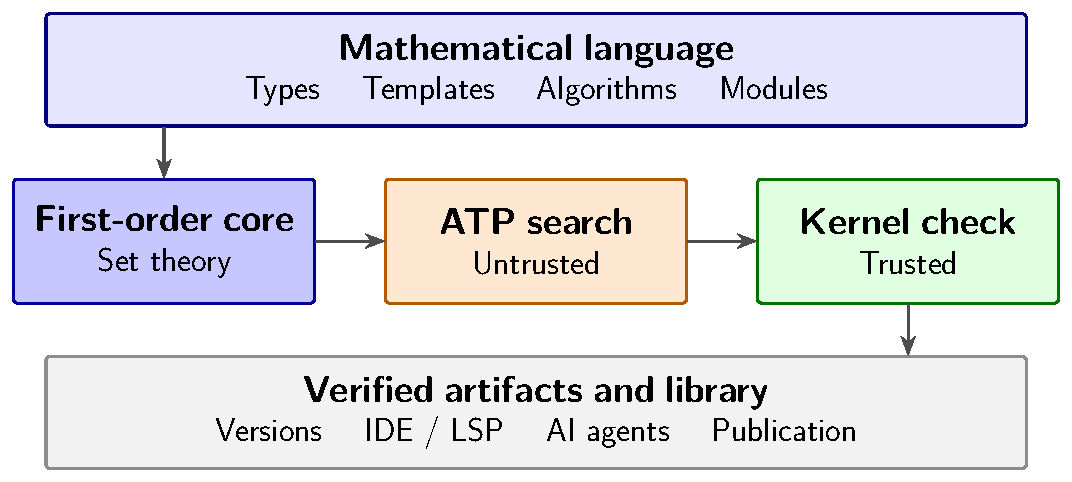
\includegraphics[width=\textwidth,height=0.64\textheight,keepaspectratio]{figures/layer_stack.pdf}
\end{center}
\begin{itemize}
\setlength{\itemsep}{1pt}
\setlength{\parsep}{0pt}
\setlength{\parskip}{0pt}
\item \textcolor{blue!55!black}{\textbf{豊かな数学的記述を、小規模な一階論理の基盤と現代的な開発環境で支える。}}
\end{itemize}
\note{
\smallskip
\textbf{Read aloud:}
\begin{itemize}
\setlength{\itemsep}{1pt}
\setlength{\parsep}{0pt}
\setlength{\parskip}{0pt}
\item \textcolor{blue!55!black}{\textbf{豊かな数学的記述を、小規模な一階論理の基盤と現代的な開発環境で支える。}}
\end{itemize}
\smallskip
\textbf{Optional notes and sources:}
\begin{itemize}
\setlength{\itemsep}{1pt}
\setlength{\parsep}{0pt}
\setlength{\parskip}{0pt}
\item 数学的な言語は elaboration を経て一階表現へ移る。外部 ATP の候補 evidence を kernel で検査し、検証済み成果物・ライブラリを IDE / LSP、AI、出版に利用する。
\end{itemize}
}
\end{frame}

\section{Part 6. Checking And Automation}
\begin{frame}[fragile,t]{6.1 - 自動化の課題: 証明探索と検査の分離}
\smallskip
\textbf{Isabelle/HOL: Sledgehammer が内部で検証する証明を提案}~\badgeSketch
\begin{lstlisting}[language={},basicstyle=\ttfamily\small]
have "Q a"
  sledgehammer
  by (metis allPQ pa)
\end{lstlisting}
\smallskip
\textbf{Mizar Evo: 引用した前提で宣言的な証明ステップを記述}~\badgeSketch
\begin{lstlisting}[language={mizar},basicstyle=\ttfamily\small]
assume AllPQ: for x being object holds P(x) implies Q(x);
assume Pa: P(a);
thus Q(a) by AllPQ, Pa;
\end{lstlisting}
\begin{itemize}
\setlength{\itemsep}{1pt}
\setlength{\parsep}{0pt}
\setlength{\parskip}{0pt}
\item \textcolor{blue!55!black}{\textbf{共通する流れ: ゴールと前提 → 外部探索 → 内側の信頼できる受理判定。prover の成功報告だけでは受理しない。}}
\item Isabelle は Metis 等で内部の証明を再構成。Mizar Evo は論理式・置換の evidence をインスタンス化し、SAT で検査する。
\end{itemize}
\note{
\smallskip
\textbf{Read aloud:}
\begin{itemize}
\setlength{\itemsep}{1pt}
\setlength{\parsep}{0pt}
\setlength{\parskip}{0pt}
\item Isabelle/HOL: Sledgehammer が内部で検証する証明を提案.
\item Mizar Evo: 引用した前提で宣言的な証明ステップを記述.
\item \textcolor{blue!55!black}{\textbf{共通する流れ: ゴールと前提 → 外部探索 → 内側の信頼できる受理判定。prover の成功報告だけでは受理しない。}}
\item Isabelle は Metis 等で内部の証明を再構成。Mizar Evo は論理式・置換の evidence をインスタンス化し、SAT で検査する。
\end{itemize}
\smallskip
\textbf{Optional notes and sources:}
\begin{itemize}
\setlength{\itemsep}{1pt}
\setlength{\parsep}{0pt}
\setlength{\parskip}{0pt}
\item Source: Sledgehammer guide (\url{https://isabelle.in.tum.de/doc/sledgehammer.pdf}), §1, 5.2; spec 16; architecture 08, 10, 15。対応する前提を仮定する説明例。
\item Evo は引用前提・局所仮定、Sledgehammer は theory context からの前提選択。共通の探索・検査の流れは evidence の同一性や実証結果を意味しない。
\end{itemize}
}
\end{frame}

\begin{frame}[fragile,t]{6.2 - ATP の活用: 探索・検査・再利用}
\begin{center}
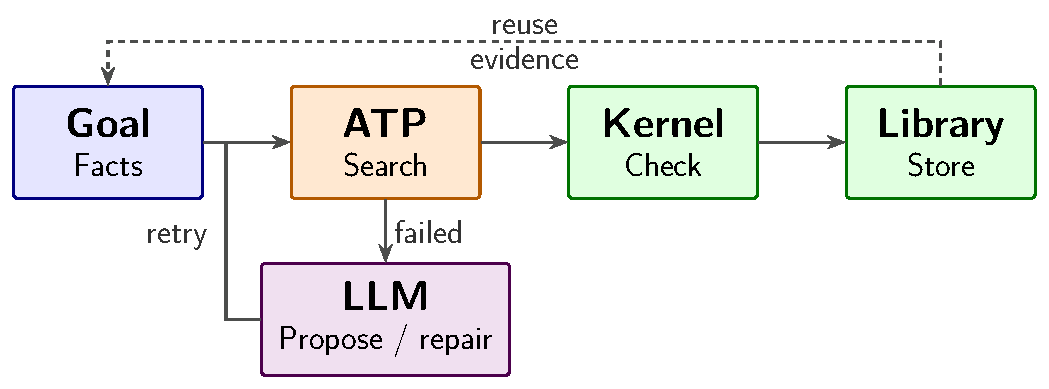
\includegraphics[width=\textwidth,height=0.54\textheight,keepaspectratio]{figures/llm_atp_loop.pdf}
\end{center}
\begin{itemize}
\setlength{\itemsep}{1pt}
\setlength{\parsep}{0pt}
\setlength{\parskip}{0pt}
\item \textcolor{blue!55!black}{\textbf{ゴールと前提 → ATP 探索 → kernel 検査 → ライブラリへ保存・再利用。}}
\item 未解決時は補題・方針を修正して再探索。図は設計意図。
\end{itemize}
\note{
\smallskip
\textbf{Read aloud:}
\begin{itemize}
\setlength{\itemsep}{1pt}
\setlength{\parsep}{0pt}
\setlength{\parskip}{0pt}
\item \textcolor{blue!55!black}{\textbf{ゴールと前提 → ATP 探索 → kernel 検査 → ライブラリへ保存・再利用。}}
\item 未解決時は補題・方針を修正して再探索。図は設計意図。
\end{itemize}
\smallskip
\textbf{Optional notes and sources:}
\begin{itemize}
\setlength{\itemsep}{1pt}
\setlength{\parsep}{0pt}
\setlength{\parskip}{0pt}
\item LLM は提案・修復を支援。受理は evidence の検査で決まり、その仕組みを次のページで示す。
\item 現在の ATP 入力は引用した前提と局所仮定。ライブラリ全体の前提選択と反復の費用対効果は今後の評価対象。
\item Source: \texttt{doc/spec/en/21.source\_code\_annotation\_and\_atp.md} §21.7.2; \texttt{doc/design/architecture/en/21.ai\_agent\_interface.md}。
\end{itemize}
}
\end{frame}

\begin{frame}[fragile,t]{6.3 - Resolution 木と置換の抽出}
\smallskip
\textbf{Resolution ログからの候補抽出}~\badgeSketch
\begin{lstlisting}[language={},basicstyle=\ttfamily\footnotesize]
F1: forall x. (P(x) implies Q(x)); F2: forall y. (Q(y) implies R(y))
H: P(a); goal: R(a); refute: F1 & F2 & H & not R(a)

{not P(x), Q(x)}             {not Q(y), R(y)}
          \                 /
           sigma1 = {x := y}       :: unify Q(x), Q(y)
           {not P(y), R(y)}        {P(a)}
                    \             /
                     sigma2 = {y := a} :: unify P(y), P(a)
                     {R(a)}        {not R(a)}
                          \        /
                           sigma3 = {}
                                {}
\end{lstlisting}
\begin{itemize}
\setlength{\itemsep}{1pt}
\setlength{\parsep}{0pt}
\setlength{\parskip}{0pt}
\item \textcolor{blue!55!black}{\textbf{非信頼の抽出器が枝上の置換を合成。F1 に \texttt{x := a}、F2 に \texttt{y := a} を保存する。}}
\end{itemize}
\note{
\smallskip
\textbf{Read aloud:}
\begin{itemize}
\setlength{\itemsep}{1pt}
\setlength{\parsep}{0pt}
\setlength{\parskip}{0pt}
\item Resolution ログからの候補抽出.
\item \textcolor{blue!55!black}{\textbf{非信頼の抽出器が枝上の置換を合成。F1 に \texttt{x := a}、F2 に \texttt{y := a} を保存する。}}
\end{itemize}
\smallskip
\textbf{Optional notes and sources:}
\begin{itemize}
\setlength{\itemsep}{1pt}
\setlength{\parsep}{0pt}
\setlength{\parskip}{0pt}
\item 節の変数 x/y は別名にしている。Q の単一化で x:=y、P の単一化で y:=a。合成して F1[x:=a] と F2[y:=a] を回収する。
\item ログを使う候補生成案。現行 architecture 10 は独立した instance finder。kernel は evidence を検査し、ログの各推論を信頼しない。
\item Source: architecture 08, 10, 15, 16。スケッチであり、外部 prover の実行例ではない。
\end{itemize}
}
\end{frame}

\begin{frame}[fragile,t]{6.3a - 保存する証拠から具体的な SAT 節へ}
\smallskip
\textbf{保存する候補・kernel の前処理・SAT 入力}~\badgeSketch
\begin{lstlisting}[language={},basicstyle=\ttfamily\footnotesize]
save: F1,F2,H (source bindings); F1[x:=a], F2[y:=a]; goal R(a), refute
check: source/context, binders, capture avoidance
instances: P(a) implies Q(a); Q(a) implies R(a); P(a); not R(a)
atoms: p=P(a)=1, q=Q(a)=2, r=R(a)=3
logical CNF: (not p or q) & (not q or r) & p & not r
Tseitin: s=4 iff (not p or q); t=5 iff (not q or r)
SAT clauses (DIMACS example; 0 ends each clause):
p cnf 5 10
1 0       -3 0
1 4 0     -2 4 0     -1 2 -4 0     4 0
2 5 0     -3 5 0     -2 3 -5 0     5 0
\end{lstlisting}
\begin{itemize}
\setlength{\itemsep}{1pt}
\setlength{\parsep}{0pt}
\setlength{\parskip}{0pt}
\item \textcolor{blue!55!black}{\textbf{small kernel が検査済み evidence から instance・CNF を生成。自身の SAT 検査器で UNSAT を確認し R(a) を受理する。外部 Resolution の各ステップは replay しない。}}
\end{itemize}
\note{
\smallskip
\textbf{Read aloud:}
\begin{itemize}
\setlength{\itemsep}{1pt}
\setlength{\parsep}{0pt}
\setlength{\parskip}{0pt}
\item 保存する候補・kernel の前処理・SAT 入力.
\item \textcolor{blue!55!black}{\textbf{small kernel が検査済み evidence から instance・CNF を生成。自身の SAT 検査器で UNSAT を確認し R(a) を受理する。外部 Resolution の各ステップは replay しない。}}
\end{itemize}
\smallskip
\textbf{Optional notes and sources:}
\begin{itemize}
\setlength{\itemsep}{1pt}
\setlength{\parsep}{0pt}
\setlength{\parskip}{0pt}
\item 元の式、合成した置換、束縛文脈、対象 VC と反駁の極性を保存。instance と SAT 節は再生成する（Backup 5）。
\item DIMACS: 5変数・10節、負の整数は否定、0 は節の終端。s/t は含意を表す。エンコーダに沿った構成例で、実行ダンプではない。
\item kernel は置換を探索しない。Source: architecture 08, 15, 16。
\end{itemize}
}
\end{frame}

\section{Status And Roadmap}
\begin{frame}[fragile,t]{仕様と実装の状況（2026年10月）}
\begin{itemize}
\setlength{\itemsep}{1pt}
\setlength{\parsep}{0pt}
\setlength{\parskip}{0pt}
\item \textcolor{blue!55!black}{\textbf{仕様: 24章と付録。英語が正典。}}
\item \textcolor{blue!55!black}{\textbf{main branch に実装済み: Rust フロントエンド（字句解析・構文解析・構文木）、alpha コーパス上の名前解決・型検査、証明義務の生成・決定的な discharge、ATP 問題の符号化・候補 evidence、SAT に基づく kernel の evidence 検査、キャッシュ・指紋・ビルドスケジューリングの各マイルストーン。}}
\item \textcolor{blue!55!black}{\textbf{進行中: ソースから検証済み成果物までの end-to-end 統合、LSP サーバ、ドキュメント生成。}}
\item \textcolor{blue!55!black}{\textbf{今後の課題: MVM 実行、コード抽出、ライブラリ全体の前提選択、MML 移行。}}
\item 本講演の対象範囲に、外部 ATP を用いた end-to-end の実証結果は含めない。
\end{itemize}
\note{
\smallskip
\textbf{Read aloud:}
\begin{itemize}
\setlength{\itemsep}{1pt}
\setlength{\parsep}{0pt}
\setlength{\parskip}{0pt}
\item \textcolor{blue!55!black}{\textbf{仕様: 24章と付録。英語が正典。}}
\item \textcolor{blue!55!black}{\textbf{main branch に実装済み: Rust フロントエンド（字句解析・構文解析・構文木）、alpha コーパス上の名前解決・型検査、証明義務の生成・決定的な discharge、ATP 問題の符号化・候補 evidence、SAT に基づく kernel の evidence 検査、キャッシュ・指紋・ビルドスケジューリングの各マイルストーン。}}
\item \textcolor{blue!55!black}{\textbf{進行中: ソースから検証済み成果物までの end-to-end 統合、LSP サーバ、ドキュメント生成。}}
\item \textcolor{blue!55!black}{\textbf{今後の課題: MVM 実行、コード抽出、ライブラリ全体の前提選択、MML 移行。}}
\item 本講演の対象範囲に、外部 ATP を用いた end-to-end の実証結果は含めない。
\end{itemize}
\smallskip
\textbf{Optional notes and sources:}
\begin{itemize}
\setlength{\itemsep}{1pt}
\setlength{\parsep}{0pt}
\setlength{\parskip}{0pt}
\item Source: \texttt{doc/design/todo.md}, Crate Status（2026年10月7日時点）。講演前に再確認。
\end{itemize}
}
\end{frame}

\begin{frame}[fragile,t]{ロードマップ}
\begin{center}
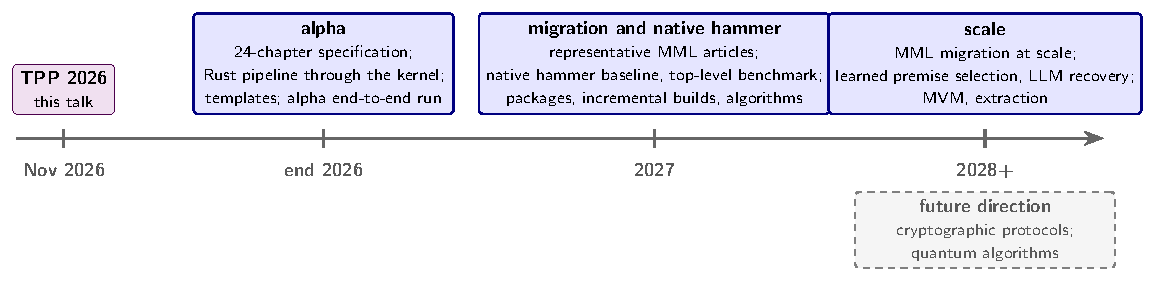
\includegraphics[width=\textwidth,height=0.44\textheight,keepaspectratio]{figures/roadmap_tpp.pdf}
\end{center}
\begin{itemize}
\setlength{\itemsep}{1pt}
\setlength{\parsep}{0pt}
\setlength{\parskip}{0pt}
\item \textcolor{blue!55!black}{\textbf{2026年: 仕様、kernel までの Rust パイプライン、template 処理、alpha の end-to-end 実行の完成。}}
\item \textcolor{blue!55!black}{\textbf{2027年: 代表的な MML article の移行、native hammer のベースライン構築、MizAR と同じ top-level theorem 単位での評価。}}
\item 2028年以降: 移行の拡大、学習ベースの前提選択、LLM による失敗回復、MVM・コード抽出。暗号・量子は将来構想。
\end{itemize}
\note{
\smallskip
\textbf{Read aloud:}
\begin{itemize}
\setlength{\itemsep}{1pt}
\setlength{\parsep}{0pt}
\setlength{\parskip}{0pt}
\item \textcolor{blue!55!black}{\textbf{2026年: 仕様、kernel までの Rust パイプライン、template 処理、alpha の end-to-end 実行の完成。}}
\item \textcolor{blue!55!black}{\textbf{2027年: 代表的な MML article の移行、native hammer のベースライン構築、MizAR と同じ top-level theorem 単位での評価。}}
\item 2028年以降: 移行の拡大、学習ベースの前提選択、LLM による失敗回復、MVM・コード抽出。暗号・量子は将来構想。
\end{itemize}
}
\end{frame}

\begin{frame}[fragile,t]{おわりに}
\begin{center}
\begin{beamercolorbox}[rounded=true,sep=2.5mm,wd=0.9\textwidth]{keyphrase}
\centering\itshape \textcolor{blue!55!black}{\textbf{Keep the foundation small.}}\\ \textcolor{blue!55!black}{\textbf{Keep the mathematics readable.}}\\ \textcolor{blue!55!black}{\textbf{Modernize everything else.}}
\end{beamercolorbox}
\end{center}
\begin{itemize}
\setlength{\itemsep}{1pt}
\setlength{\parsep}{0pt}
\setlength{\parskip}{0pt}
\item \textcolor{blue!55!black}{\textbf{基盤を小さく保ち、数学的記述の可読性を維持し、周辺基盤を現代化する。}}
\item \textcolor{blue!55!black}{\textbf{議論したい点: MML の移行、記述の利便性、自動化の評価。}}
\end{itemize}
\note{
\smallskip
\textbf{Read aloud:}
\begin{itemize}
\setlength{\itemsep}{1pt}
\setlength{\parsep}{0pt}
\setlength{\parskip}{0pt}
\item \textcolor{blue!55!black}{\textbf{Keep the foundation small.}} \textcolor{blue!55!black}{\textbf{Keep the mathematics readable.}} \textcolor{blue!55!black}{\textbf{Modernize everything else.}}
\item \textcolor{blue!55!black}{\textbf{基盤を小さく保ち、数学的記述の可読性を維持し、周辺基盤を現代化する。}}
\item \textcolor{blue!55!black}{\textbf{議論したい点: MML の移行、記述の利便性、自動化の評価。}}
\end{itemize}
}
\end{frame}

\appendix
\section{Backup 1. MizAR 60 の詳細}
\begin{frame}[fragile,t]{Backup 1. MizAR 60 の詳細}
Source: Jakubův et al., MizAR 60 for Mizar 50, ITP 2023.

\begin{itemize}
\setlength{\itemsep}{1pt}
\setlength{\parsep}{0pt}
\setlength{\parskip}{0pt}
\item データ: MPTP で出力した MML 1147、無名の top-level lemma を含む 57,897 件の定理。MizAR 40 と同一版を用いた比較。
\item 学習・開発・holdout を90:5:5に分割。holdout 2,896件中1,690件（58.4\%）を hammering mode で証明。ユーザの前提指定なし、420 CPU 秒（MizAR 40 は約40.6\%）。
\item 人または機械がライブラリから前提を選べる条件では 75\% 超（MizAR 40 は 56\%）。
\item 最高性能の単一手法: hammering mode で 30 秒 40\%。人間の前提指定ありで 120 秒 60\%。
\item 転移: 同手法を MML 1382 の新規 242 article、13,370 定理にも適用。
\item 手法: ENIGMA と Deepire で誘導した E と Vampire、学習ベースの前提選択、数百万の ATP 証明で学習するループ。
\end{itemize}
\note{
\smallskip
\textbf{Read aloud:}
\begin{itemize}
\setlength{\itemsep}{1pt}
\setlength{\parsep}{0pt}
\setlength{\parskip}{0pt}
\item データ: MPTP で出力した MML 1147、無名の top-level lemma を含む 57,897 件の定理。MizAR 40 と同一版を用いた比較。
\item 学習・開発・holdout を90:5:5に分割。holdout 2,896件中1,690件（58.4\%）を hammering mode で証明。ユーザの前提指定なし、420 CPU 秒（MizAR 40 は約40.6\%）。
\item 人または機械がライブラリから前提を選べる条件では 75\% 超（MizAR 40 は 56\%）。
\item 最高性能の単一手法: hammering mode で 30 秒 40\%。人間の前提指定ありで 120 秒 60\%。
\item 転移: 同手法を MML 1382 の新規 242 article、13,370 定理にも適用。
\item 手法: ENIGMA と Deepire で誘導した E と Vampire、学習ベースの前提選択、数百万の ATP 証明で学習するループ。
\end{itemize}
\smallskip
\textbf{Optional notes and sources:}
\begin{itemize}
\setlength{\itemsep}{1pt}
\setlength{\parsep}{0pt}
\setlength{\parskip}{0pt}
\item Source: Jakubův et al., MizAR 60 for Mizar 50, ITP 2023.
\end{itemize}
}
\end{frame}

\section{Backup 2. Sledgehammer 評価の詳細}
\begin{frame}[fragile,t]{Backup 2. Sledgehammer 評価の詳細}
\begin{footnotesize}
\setlength{\tabcolsep}{3pt}
\renewcommand{\arraystretch}{1.15}
\begin{tabularx}{\textwidth}{>{\raggedright\arraybackslash}X>{\raggedright\arraybackslash}X>{\raggedright\arraybackslash}X}
\toprule
\textbf{評価} & \textbf{対象・方式} & \textbf{成功率} \\
\midrule
ITP 2022 & AFP 5,000ゴール、greedy 16構成 & 68.8\% \\
Magnushammer（2023年公開） & PISA 1,000定理、Sledgehammer & 38.3\% \\
同じ PISA 評価 & 学習による前提選択を用いる Magnushammer & 59.5\% \\
\bottomrule
\end{tabularx}
\end{footnotesize}

\begin{itemize}
\setlength{\itemsep}{1pt}
\setlength{\parsep}{0pt}
\setlength{\parskip}{0pt}
\item ITP 2022: 50 entry × 100ゴール。MePo、基準512事実、各構成30 CPU 秒。構成は評価集合から事後選択。再構成は評価対象外。
\item PISA: Isabelle2021-1、Sledgehammer の timeout 30秒、ローカル5 prover、複数設定の成功集合を集約。Isabelle 内での検証を成功条件とする。
\item 年代が近くても、局所ゴールと定理全体、探索成功と検証済み証明を混同しない。
\end{itemize}
\note{
\smallskip
\textbf{Read aloud:}
\begin{itemize}
\setlength{\itemsep}{1pt}
\setlength{\parsep}{0pt}
\setlength{\parskip}{0pt}
\item ITP 2022: 50 entry × 100ゴール。MePo、基準512事実、各構成30 CPU 秒。構成は評価集合から事後選択。再構成は評価対象外。
\item PISA: Isabelle2021-1、Sledgehammer の timeout 30秒、ローカル5 prover、複数設定の成功集合を集約。Isabelle 内での検証を成功条件とする。
\item 年代が近くても、局所ゴールと定理全体、探索成功と検証済み証明を混同しない。
\end{itemize}
\smallskip
\textbf{Optional notes and sources:}
\begin{itemize}
\setlength{\itemsep}{1pt}
\setlength{\parsep}{0pt}
\setlength{\parskip}{0pt}
\item Source: Desharnais et al., Seventeen Provers Under the Hammer, ITP 2022, sections 5, 5.6, Table 10; Miku\l{}a et al., Magnushammer, arXiv:2303.04488（2023年公開）, Table 2, Appendix A.4。
\end{itemize}
}
\end{frame}

\section{Backup 3. HOL から FOL への符号化と再構成}
\begin{frame}[fragile,t]{Backup 3. HOL から FOL への符号化と再構成}
\begin{itemize}
\setlength{\itemsep}{1pt}
\setlength{\parsep}{0pt}
\setlength{\parskip}{0pt}
\item 関数適用: 関数変数の適用を \texttt{app(F, X)} で表現。定数の適用はカリー化を維持、または平坦化。
\item ラムダ抽象: lambda lifting は定義式付きの新しい定数を導入する。コンビネータ変換が代替。
\item 型: 多相な HOL の型を guard、tag、または単相化で符号化。選択は健全性・完全性・prover 性能に影響する。
\item 真偽値: 論理式中の真偽値を返す項には追加の符号化が必要。
\item 再構成: 使用した補題による \texttt{metis}、SMT 証明の \texttt{smt} replay、生成した Isar テキスト。再構成の失敗は別途集計。
\end{itemize}
Source: Meng and Paulson 2008; Blanchette, Böhme, Popescu, Smallbone 2016; Blanchette, Kaliszyk, Paulson, Urban 2016; Schurr, Fleury, Desharnais 2021.

\note{
\smallskip
\textbf{Read aloud:}
\begin{itemize}
\setlength{\itemsep}{1pt}
\setlength{\parsep}{0pt}
\setlength{\parskip}{0pt}
\item 関数適用: 関数変数の適用を \texttt{app(F, X)} で表現。定数の適用はカリー化を維持、または平坦化。
\item ラムダ抽象: lambda lifting は定義式付きの新しい定数を導入する。コンビネータ変換が代替。
\item 型: 多相な HOL の型を guard、tag、または単相化で符号化。選択は健全性・完全性・prover 性能に影響する。
\item 真偽値: 論理式中の真偽値を返す項には追加の符号化が必要。
\item 再構成: 使用した補題による \texttt{metis}、SMT 証明の \texttt{smt} replay、生成した Isar テキスト。再構成の失敗は別途集計。
\end{itemize}
\smallskip
\textbf{Optional notes and sources:}
\begin{itemize}
\setlength{\itemsep}{1pt}
\setlength{\parsep}{0pt}
\setlength{\parskip}{0pt}
\item Source: Meng and Paulson 2008; Blanchette, Böhme, Popescu, Smallbone 2016; Blanchette, Kaliszyk, Paulson, Urban 2016; Schurr, Fleury, Desharnais 2021.
\end{itemize}
}
\end{frame}

\section{Backup 4. Template のインスタンス化: 一つの証明、多くのビュー}
\begin{frame}[fragile,t]{Backup 4. Template のインスタンス化: 一つの証明、多くのビュー}
\smallskip
\textbf{有界な型パラメータと汎用的な定理}~\badgeSpec~{\footnotesize(証明は省略)}
\begin{lstlisting}[language={mizar},basicstyle=\ttfamily\footnotesize]
definition
  let T be type extends commutative associative unital Magma;
  theorem PermProduct[T]:
    for s being FinSequence of T,
        p being Permutation of dom s
    holds Product[T](s) = Product[T](s * p)
  proof ... end;
end;
\end{lstlisting}
\smallskip
\textbf{インスタンス化}~\badgeSpec~{\footnotesize(必要な registration がある前提)}
\begin{lstlisting}[language={mizar},basicstyle=\ttfamily\small]
PermProduct[commutative associative unital AddMagma]
PermProduct[commutative associative unital MulMagma]
let R be commutative Ring;  PermProduct[R qua AddMagma]  :: additive view
\end{lstlisting}
\begin{itemize}
\setlength{\itemsep}{1pt}
\setlength{\parsep}{0pt}
\setlength{\parskip}{0pt}
\item 環から Magma への継承経路は二つ。\texttt{qua} によるビューの選択が、記法を決定する。
\end{itemize}
\note{
\smallskip
\textbf{Read aloud:}
\begin{itemize}
\setlength{\itemsep}{1pt}
\setlength{\parsep}{0pt}
\setlength{\parskip}{0pt}
\item 有界な型パラメータと汎用的な定理.
\item インスタンス化.
\item 環から Magma への継承経路は二つ。\texttt{qua} によるビューの選択が、記法を決定する。
\end{itemize}
\smallskip
\textbf{Optional notes and sources:}
\begin{itemize}
\setlength{\itemsep}{1pt}
\setlength{\parsep}{0pt}
\setlength{\parskip}{0pt}
\item Source: \texttt{doc/spec/en/18.templates.md}, section 18.2.2.
\end{itemize}
}
\end{frame}

\section{Backup 5. Kernel evidence と信頼できる SAT 検査}
\begin{frame}[fragile,t]{Backup 5. Kernel evidence と信頼できる SAT 検査}
\begin{center}
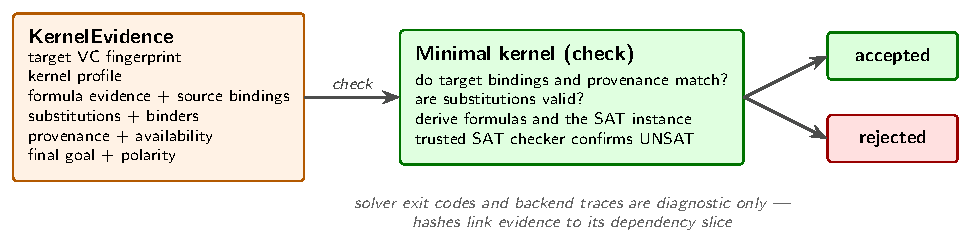
\includegraphics[width=\textwidth,height=0.52\textheight,keepaspectratio]{../2026-09-bialystok/figures/certificate_replay.pdf}
\end{center}
\begin{itemize}
\setlength{\itemsep}{1pt}
\setlength{\parsep}{0pt}
\setlength{\parskip}{0pt}
\item evidence は元の論理式・明示的な代入・来歴・対象とゴールの対応を保持。kernel はこれらを検査し、決定的な SAT 問題を生成。信頼できるプロセス内 SAT 検査器で UNSAT を確認する。
\item バックエンドの証明トレース、SMT の証明オブジェクト、ログ、終了コードは診断用のみ。
\end{itemize}
\note{
\smallskip
\textbf{Read aloud:}
\begin{itemize}
\setlength{\itemsep}{1pt}
\setlength{\parsep}{0pt}
\setlength{\parskip}{0pt}
\item evidence は元の論理式・明示的な代入・来歴・対象とゴールの対応を保持。kernel はこれらを検査し、決定的な SAT 問題を生成。信頼できるプロセス内 SAT 検査器で UNSAT を確認する。
\item バックエンドの証明トレース、SMT の証明オブジェクト、ログ、終了コードは診断用のみ。
\end{itemize}
\smallskip
\textbf{Optional notes and sources:}
\begin{itemize}
\setlength{\itemsep}{1pt}
\setlength{\parsep}{0pt}
\setlength{\parskip}{0pt}
\item Source: \texttt{doc/design/architecture/en/08.reasoning\_boundary.md}, \texttt{15.kernel\_certificate\_format.md}.
\end{itemize}
}
\end{frame}

\section{Backup 6. ATP の中心経路}
\begin{frame}[fragile,t]{Backup 6. ATP の中心経路}
\begin{center}
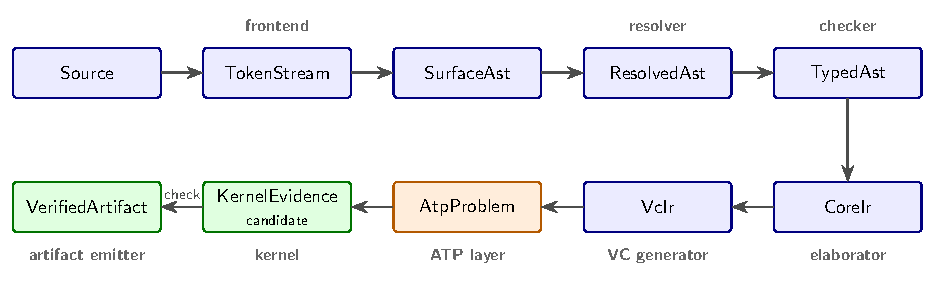
\includegraphics[width=\textwidth,height=0.52\textheight,keepaspectratio]{../2026-09-bialystok/figures/pipeline.pdf}
\end{center}
\begin{itemize}
\setlength{\itemsep}{1pt}
\setlength{\parsep}{0pt}
\setlength{\parskip}{0pt}
\item 決定的な discharge 後の未解決義務のみを ATP に送る。前段の discharge にも再検査可能な evidence が必要。
\item 各境界で、情報の管理主体・記録する成果物・変更後の再検査範囲を定める。
\end{itemize}
\note{
\smallskip
\textbf{Read aloud:}
\begin{itemize}
\setlength{\itemsep}{1pt}
\setlength{\parsep}{0pt}
\setlength{\parskip}{0pt}
\item 決定的な discharge 後の未解決義務のみを ATP に送る。前段の discharge にも再検査可能な evidence が必要。
\item 各境界で、情報の管理主体・記録する成果物・変更後の再検査範囲を定める。
\end{itemize}
\smallskip
\textbf{Optional notes and sources:}
\begin{itemize}
\setlength{\itemsep}{1pt}
\setlength{\parsep}{0pt}
\setlength{\parskip}{0pt}
\item Source: \texttt{doc/design/architecture/en/00.pipeline\_overview.md}; Bia\l{}ystok 資料 Part 10。
\end{itemize}
}
\end{frame}

\section{Backup 7. 差分検証}
\begin{frame}[fragile,t]{Backup 7. 差分検証}
\begin{center}
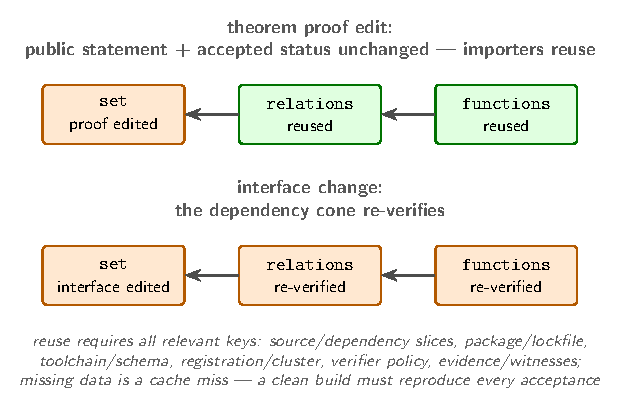
\includegraphics[width=\textwidth,height=0.52\textheight,keepaspectratio]{../2026-09-bialystok/figures/fingerprint_graph.pdf}
\end{center}
\begin{itemize}
\setlength{\itemsep}{1pt}
\setlength{\parsep}{0pt}
\setlength{\parskip}{0pt}
\item 証明本体の編集時、公開された主張と受理状態が不変なら、依存側の再ビルドは不要。インタフェース変更時は依存コーンを再検証。
\item キャッシュ再利用には、関連キーの完全一致が必要。データ欠落時はキャッシュミス。再利用自体は証明の正当性を保証せず、クリーンビルドで全受理結果を再現する。
\end{itemize}
\note{
\smallskip
\textbf{Read aloud:}
\begin{itemize}
\setlength{\itemsep}{1pt}
\setlength{\parsep}{0pt}
\setlength{\parskip}{0pt}
\item 証明本体の編集時、公開された主張と受理状態が不変なら、依存側の再ビルドは不要。インタフェース変更時は依存コーンを再検証。
\item キャッシュ再利用には、関連キーの完全一致が必要。データ欠落時はキャッシュミス。再利用自体は証明の正当性を保証せず、クリーンビルドで全受理結果を再現する。
\end{itemize}
\smallskip
\textbf{Optional notes and sources:}
\begin{itemize}
\setlength{\itemsep}{1pt}
\setlength{\parsep}{0pt}
\setlength{\parskip}{0pt}
\item Source: \texttt{doc/design/architecture/en/11.artifact\_and\_incremental\_build.md}, \texttt{18.dependency\_fingerprint.md}; Bia\l{}ystok 資料 Story 5。
\end{itemize}
}
\end{frame}

\section{Backup 8. Package manifest}
\begin{frame}[fragile,t]{Backup 8. Package manifest}
\smallskip
\textbf{Mizar Evo}~\badgeSpec
\begin{lstlisting}[language={toml},basicstyle=\ttfamily\footnotesize]
[package]
name    = "algebra"
version = "2.3.1"
edition = "2025"

[dependencies]
mml_core = "^1.0"
topology = { version = "^0.9", features = ["metric"] }
\end{lstlisting}
\begin{itemize}
\setlength{\itemsep}{1pt}
\setlength{\parsep}{0pt}
\setlength{\parskip}{0pt}
\item 再現可能なビルドの要件: 固定したソース・lockfile・ツールチェーン・検査器設定・決定的な ATP evidence。
\item バージョン管理された再利用により、article 集合間の手作業コピーを解消。集約モジュールで、一分野を一つの import として公開できる。
\end{itemize}
Source: \texttt{doc/spec/en/23.package\_management\_and\_build\_system.md}; Bia\l{}ystok 資料 Story 1。

\note{
\smallskip
\textbf{Read aloud:}
\begin{itemize}
\setlength{\itemsep}{1pt}
\setlength{\parsep}{0pt}
\setlength{\parskip}{0pt}
\item 再現可能なビルドの要件: 固定したソース・lockfile・ツールチェーン・検査器設定・決定的な ATP evidence。
\item バージョン管理された再利用により、article 集合間の手作業コピーを解消。集約モジュールで、一分野を一つの import として公開できる。
\end{itemize}
\smallskip
\textbf{Optional notes and sources:}
\begin{itemize}
\setlength{\itemsep}{1pt}
\setlength{\parsep}{0pt}
\setlength{\parskip}{0pt}
\item Source: \texttt{doc/spec/en/23.package\_management\_and\_build\_system.md}; Bia\l{}ystok 資料 Story 1。
\end{itemize}
}
\end{frame}

\section{Backup 9. 45分版での追加}
\begin{frame}[fragile,t]{Backup 9. 45分版での追加}
\smallskip
\textbf{時間に応じ、以下の具体例を追加:}
\begin{enumerate}
\setlength{\itemsep}{1pt}
\setlength{\parsep}{0pt}
\setlength{\parskip}{0pt}
\item 単一のゴールで HOL から FOL への関数の符号化を説明（\texttt{app}、部分適用、lambda lifting）。
\item Mizar の関数表現: \texttt{Function of X,Y}、\texttt{f.x}、集合論的対象としての soft type。
\item Template: 加法と乗法のビューを持つ \texttt{PermProduct[T]}（Backup 4）。
\item Algorithm: ユークリッドの互除法、\texttt{by computation}、関数子への昇格。
\item Structure とビュー: \texttt{AddMagma}、\texttt{MulMagma}、\texttt{Magma}（Bia\l{}ystok Story 2）。
\item 現代的な基盤: \texttt{mizar.pkg}、namespace、指紋グラフ（Backup 7-8）。
\item 検査: evidence のインスタンス化と SAT 検査（本編 6.3、詳細は Backup 5）。
\end{enumerate}
\note{
\smallskip
\textbf{Read aloud:}
\begin{itemize}
\setlength{\itemsep}{1pt}
\setlength{\parsep}{0pt}
\setlength{\parskip}{0pt}
\item 単一のゴールで HOL から FOL への関数の符号化を説明（\texttt{app}、部分適用、lambda lifting）。
\item Mizar の関数表現: \texttt{Function of X,Y}、\texttt{f.x}、集合論的対象としての soft type。
\item Template: 加法と乗法のビューを持つ \texttt{PermProduct[T]}（Backup 4）。
\item Algorithm: ユークリッドの互除法、\texttt{by computation}、関数子への昇格。
\item Structure とビュー: \texttt{AddMagma}、\texttt{MulMagma}、\texttt{Magma}（Bia\l{}ystok Story 2）。
\item 現代的な基盤: \texttt{mizar.pkg}、namespace、指紋グラフ（Backup 7-8）。
\item 検査: evidence のインスタンス化と SAT 検査（本編 6.3、詳細は Backup 5）。
\end{itemize}
}
\end{frame}

\section{Backup 10. 出典と帰属}
\begin{frame}[fragile,t]{Backup 10. 出典と帰属}
\smallskip
\textbf{本講演における MML の原文引用:}
\begin{scriptsize}
\setlength{\tabcolsep}{3pt}
\renewcommand{\arraystretch}{1.15}
\begin{tabularx}{\textwidth}{>{\raggedright\arraybackslash}X>{\raggedright\arraybackslash}X>{\raggedright\arraybackslash}X>{\raggedright\arraybackslash}X}
\toprule
\textbf{目的} & \textbf{出典} & \textbf{行} & \textbf{使用箇所} \\
\midrule
関数適用 \texttt{f.x} & \texttt{funct\_1.miz} & 138-140 & Frame 1.2 \\
soft type としての \texttt{Function of X,Y} & \texttt{funct\_2.miz} & 87-90 & Frame 1.2 \\
\bottomrule
\end{tabularx}
\end{scriptsize}

\smallskip
\textbf{Source URLs:}
\begin{itemize}
\setlength{\itemsep}{1pt}
\setlength{\parsep}{0pt}
\setlength{\parskip}{0pt}
\item \texttt{FUNCT\_1}: \url{https://mizar.uwb.edu.pl/version/current/mml/funct\_1.miz}
\item \texttt{FUNCT\_2}: \url{https://mizar.uwb.edu.pl/version/current/mml/funct\_2.miz}
\end{itemize}
\smallskip
\textbf{帰属についての注記:}
\begin{itemize}
\setlength{\itemsep}{1pt}
\setlength{\parsep}{0pt}
\setlength{\parskip}{0pt}
\item MML のテキストは GPL-3.0-or-later / CC-BY-SA-3.0-or-later。article 名・URL・行番号を発表者ノートに記載。
\item ベンチマークの数値は Backup 1-2 と \texttt{references.bib} を参照。最終版の作成前に、出版社の情報で書誌事項を確認。
\end{itemize}
\note{
\smallskip
\textbf{Read aloud:}
\begin{itemize}
\setlength{\itemsep}{1pt}
\setlength{\parsep}{0pt}
\setlength{\parskip}{0pt}
\item \texttt{FUNCT\_1}: \url{https://mizar.uwb.edu.pl/version/current/mml/funct\_1.miz}
\item \texttt{FUNCT\_2}: \url{https://mizar.uwb.edu.pl/version/current/mml/funct\_2.miz}
\item MML のテキストは GPL-3.0-or-later / CC-BY-SA-3.0-or-later。article 名・URL・行番号を発表者ノートに記載。
\item ベンチマークの数値は Backup 1-2 と \texttt{references.bib} を参照。最終版の作成前に、出版社の情報で書誌事項を確認。
\end{itemize}
}
\end{frame}

\section{Backup 11. 評価条件の比較}
\begin{frame}[fragile,t]{Backup 11. 評価条件の比較}
\begin{scriptsize}
\setlength{\tabcolsep}{3pt}
\renewcommand{\arraystretch}{1.15}
\begin{tabularx}{\textwidth}{>{\raggedright\arraybackslash}X>{\raggedright\arraybackslash}X>{\raggedright\arraybackslash}X}
\toprule
\textbf{} & \textbf{MizAR 60 (ITP 2023)} & \textbf{Sledgehammer / AFP (ITP 2022)} \\
\midrule
報告された成功率 & 58.4\%（1,690 / 2,896） & 68.8\%（3,440 / 5,000） \\
評価対象 & MML 1147 の定理・補題。全57,897件のうち holdout 2,896件 & AFP の50 entry から選んだ局所ゴール5,000件 \\
前提選択 & ライブラリ全体から学習的に選択 & MePo。基準512事実、構成により増減 \\
時間予算 & ポートフォリオ合計 420 CPU 秒 & greedy 16構成 × 各30 CPU 秒 = 480 CPU 秒 \\
成功の判定 & ATP 証明の発見（hammering mode） & 外部 prover の証明発見。Isabelle 内の再構成は評価対象外 \\
\bottomrule
\end{tabularx}
\end{scriptsize}

\begin{itemize}
\setlength{\itemsep}{1pt}
\setlength{\parsep}{0pt}
\setlength{\parskip}{0pt}
\item \textcolor{blue!55!black}{\textbf{評価対象・前提選択・時間予算・構成選択が異なる。成功率だけでは設計上の優劣を判定できない。}}
\end{itemize}
\note{
\smallskip
\textbf{Read aloud:}
\begin{itemize}
\setlength{\itemsep}{1pt}
\setlength{\parsep}{0pt}
\setlength{\parskip}{0pt}
\item \textcolor{blue!55!black}{\textbf{評価対象・前提選択・時間予算・構成選択が異なる。成功率だけでは設計上の優劣を判定できない。}}
\end{itemize}
\smallskip
\textbf{Optional notes and sources:}
\begin{itemize}
\setlength{\itemsep}{1pt}
\setlength{\parsep}{0pt}
\setlength{\parskip}{0pt}
\item 「ハンマー」は goal を自動証明器に送る道具。「前提」は prover が使ってよい事実。
\item Source: Jakubův et al. 2023, sections 6.2, 6.5; Desharnais et al. 2022, sections 5, 5.6, Table 10（greedy 構成は同じ評価集合から事後選択）。
\item 公表年と実験時期は異なる。MizAR の主要実験は2020–2021年。AFP 評価は2022年1月の Isabelle と2021年12月の AFP を使用。
\item MizAR の 75\% は、人または機械がライブラリから前提を選んだ条件。質問用に取っておく。
\end{itemize}
}
\end{frame}

\section{Backup 12. 評価単位: 定理全体と局所ゴール}
\begin{frame}[fragile,t]{Backup 12. 評価単位: 定理全体と局所ゴール}
\begin{center}
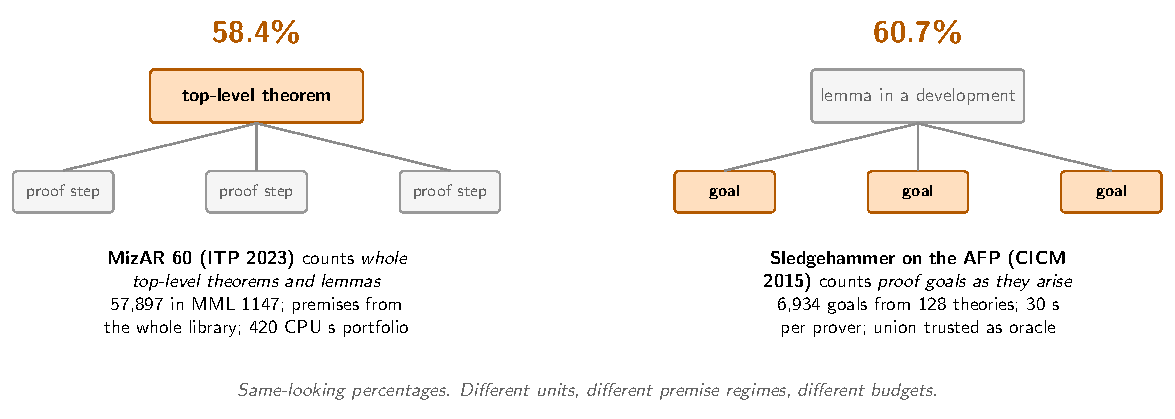
\includegraphics[width=\textwidth,height=0.48\textheight,keepaspectratio]{figures/evaluation_units.pdf}
\end{center}
\begin{itemize}
\setlength{\itemsep}{1pt}
\setlength{\parsep}{0pt}
\setlength{\parskip}{0pt}
\item \textcolor{blue!55!black}{\textbf{MizAR: 著者による前提指定なしに、ライブラリから定理全体を自動証明できるか。}}
\item \textcolor{blue!55!black}{\textbf{AFP 研究: 証明中の局所ゴールを、その文脈で自動証明できるか。多くは人手で記述された証明の内部に位置する。}}
\item いずれも妥当な評価であるが、対象とする課題は異なる。
\end{itemize}
\note{
\smallskip
\textbf{Read aloud:}
\begin{itemize}
\setlength{\itemsep}{1pt}
\setlength{\parsep}{0pt}
\setlength{\parskip}{0pt}
\item \textcolor{blue!55!black}{\textbf{MizAR: 著者による前提指定なしに、ライブラリから定理全体を自動証明できるか。}}
\item \textcolor{blue!55!black}{\textbf{AFP 研究: 証明中の局所ゴールを、その文脈で自動証明できるか。多くは人手で記述された証明の内部に位置する。}}
\item いずれも妥当な評価であるが、対象とする課題は異なる。
\end{itemize}
}
\end{frame}

\section{Backup 13. 一階 ATP への二つの接続経路}
\begin{frame}[fragile,t]{Backup 13. 一階 ATP への二つの接続経路}
\begin{center}
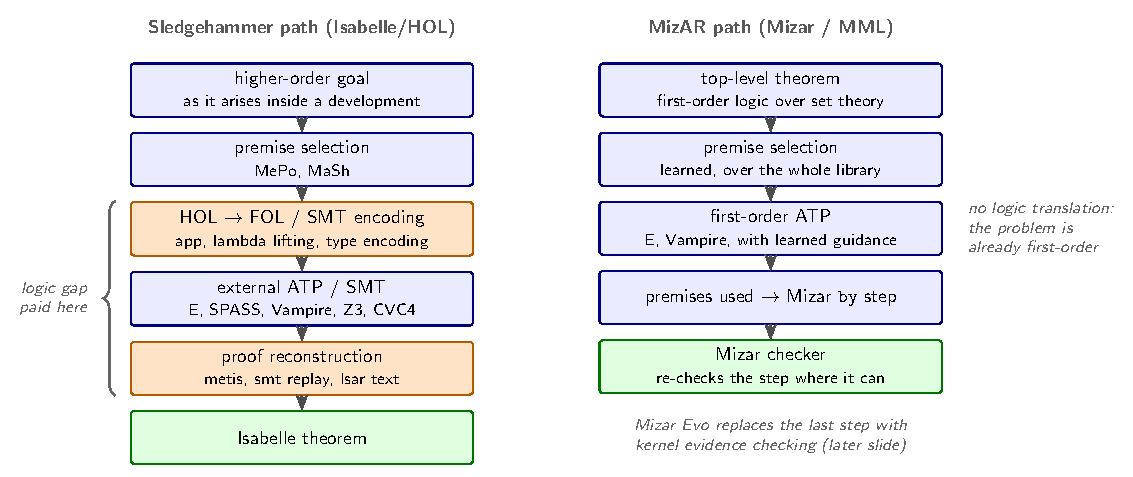
\includegraphics[width=\textwidth,height=0.56\textheight,keepaspectratio]{figures/two_paths.pdf}
\end{center}
\begin{itemize}
\setlength{\itemsep}{1pt}
\setlength{\parsep}{0pt}
\setlength{\parskip}{0pt}
\item \textcolor{blue!55!black}{\textbf{Sledgehammer の一階・SMT 経路: 高階のゴールを翻訳し、得られた証明を Isabelle 内で再構成する。}}
\item \textcolor{blue!55!black}{\textbf{MizAR: 一階・集合論の問題を ATP へ送る。}}
\end{itemize}
\note{
\smallskip
\textbf{Read aloud:}
\begin{itemize}
\setlength{\itemsep}{1pt}
\setlength{\parsep}{0pt}
\setlength{\parskip}{0pt}
\item \textcolor{blue!55!black}{\textbf{Sledgehammer の一階・SMT 経路: 高階のゴールを翻訳し、得られた証明を Isabelle 内で再構成する。}}
\item \textcolor{blue!55!black}{\textbf{MizAR: 一階・集合論の問題を ATP へ送る。}}
\end{itemize}
\smallskip
\textbf{Optional notes and sources:}
\begin{itemize}
\setlength{\itemsep}{1pt}
\setlength{\parsep}{0pt}
\setlength{\parskip}{0pt}
\item どちらも既存システムの説明（Blanchette, Kaliszyk, Paulson, Urban 2016; Jakubův et al. 2023）。オレンジの箱が翻訳と再構成の層。
\item 図は一階・SMT 接続の概形。ITP 2022 の評価は、高階形式を直接扱う prover も含む。
\item MizAR の見出しの数字は ATP 証明を数える。Mizar checker は、推論が検査器の強さの範囲なら、得られた \texttt{by} ステップを再検査する。
\end{itemize}
}
\end{frame}

\section{Backup 14. 高階論理における関数}
\begin{frame}[fragile,t]{Backup 14. 高階論理における関数}
\smallskip
\textbf{HOL の文の概形}~\badgeSketch~{\footnotesize(Isabelle/HOL 風の記法)}
\begin{lstlisting}[language={},basicstyle=\ttfamily\small]
f :: 'a => 'b        x :: 'a

P (f x)
\end{lstlisting}
\begin{itemize}
\setlength{\itemsep}{1pt}
\setlength{\parsep}{0pt}
\setlength{\parskip}{0pt}
\item \textcolor{blue!55!black}{\textbf{HOL: 関数型と関数適用を論理に組み込む。}}
\item 関数を引数・戻り値とする関数、部分適用、ラムダ抽象を直接記述できる。
\item \textcolor{blue!55!black}{\textbf{高階の構造を用いた簡潔な数学的記述が可能。}}
\item \textcolor{blue!55!black}{\textbf{E や Vampire の一階推論を利用するには、高階構造を一階表現へ符号化する必要がある。}}
\end{itemize}
\note{
\smallskip
\textbf{Read aloud:}
\begin{itemize}
\setlength{\itemsep}{1pt}
\setlength{\parsep}{0pt}
\setlength{\parskip}{0pt}
\item HOL の文の概形.
\item \textcolor{blue!55!black}{\textbf{HOL: 関数型と関数適用を論理に組み込む。}}
\item 関数を引数・戻り値とする関数、部分適用、ラムダ抽象を直接記述できる。
\item \textcolor{blue!55!black}{\textbf{高階の構造を用いた簡潔な数学的記述が可能。}}
\item \textcolor{blue!55!black}{\textbf{E や Vampire の一階推論を利用するには、高階構造を一階表現へ符号化する必要がある。}}
\end{itemize}
}
\end{frame}

\section{Backup 15. HOL の符号化と再構成}
\begin{frame}[fragile,t]{Backup 15. HOL の符号化と再構成}
\smallskip
\textbf{符号化の手順の概形}~\badgeSketch
\begin{lstlisting}[language={},basicstyle=\ttfamily\footnotesize]
F X                   ->  app(F, X)
(%x. t) ...           ->  fresh constant + defining axioms   (lambda lifting)
polymorphic types     ->  type guards or type tags
Boolean-valued terms  ->  extra encoding
\end{lstlisting}
\begin{itemize}
\setlength{\itemsep}{1pt}
\setlength{\parsep}{0pt}
\setlength{\parskip}{0pt}
\item \textcolor{blue!55!black}{\textbf{関数変数の適用は \texttt{app} で明示。ラムダ抽象は lambda lifting またはコンビネータで、型は guard または tag で符号化する。}}
\item \textcolor{blue!55!black}{\textbf{ATP の証明を Isabelle 内で再構成（reconstruction）: \texttt{metis}、\texttt{smt} の replay、生成した Isar テキストを利用。}}
\item 高階 ITP と一階 ATP の接続を実現する技術。
\item 接続の仕組みを示す説明であり、実測上の性能の優劣を示すものではない。
\end{itemize}
\note{
\smallskip
\textbf{Read aloud:}
\begin{itemize}
\setlength{\itemsep}{1pt}
\setlength{\parsep}{0pt}
\setlength{\parskip}{0pt}
\item 符号化の手順の概形.
\item \textcolor{blue!55!black}{\textbf{関数変数の適用は \texttt{app} で明示。ラムダ抽象は lambda lifting またはコンビネータで、型は guard または tag で符号化する。}}
\item \textcolor{blue!55!black}{\textbf{ATP の証明を Isabelle 内で再構成（reconstruction）: \texttt{metis}、\texttt{smt} の replay、生成した Isar テキストを利用。}}
\item 高階 ITP と一階 ATP の接続を実現する技術。
\item 接続の仕組みを示す説明であり、実測上の性能の優劣を示すものではない。
\end{itemize}
\smallskip
\textbf{Optional notes and sources:}
\begin{itemize}
\setlength{\itemsep}{1pt}
\setlength{\parsep}{0pt}
\setlength{\parskip}{0pt}
\item Source: Meng and Paulson 2008（高階節から一階節への翻訳）; Blanchette, Böhme, Popescu, Smallbone 2016（型の符号化）; Blanchette, Kaliszyk, Paulson, Urban 2016（サーベイ）; Schurr, Fleury, Desharnais 2021（再構成）。
\item Sledgehammer が実際に使う符号化は prover とオプションで変わる。この枚は概形。
\end{itemize}
}
\end{frame}

\section{Backup 16. 複雑さを担う層の違い}
\begin{frame}[fragile,t]{Backup 16. 複雑さを担う層の違い}
\begin{center}
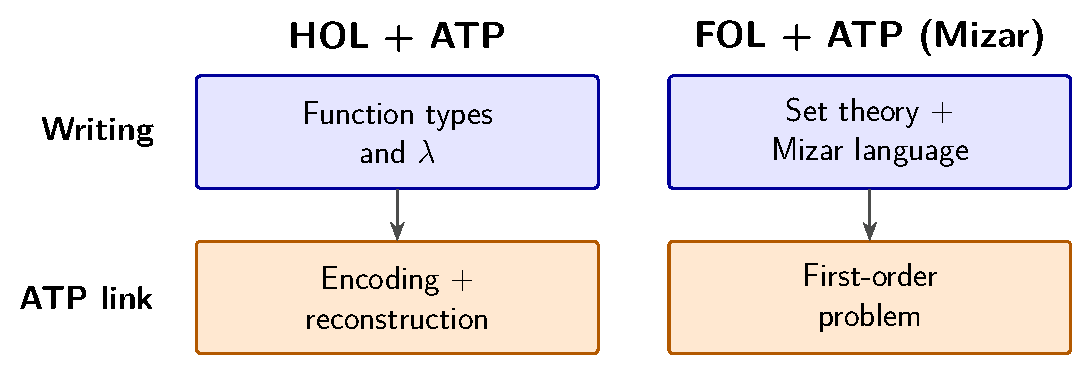
\includegraphics[width=\textwidth,height=0.54\textheight,keepaspectratio]{figures/where_you_pay.pdf}
\end{center}
\begin{itemize}
\setlength{\itemsep}{1pt}
\setlength{\parsep}{0pt}
\setlength{\parskip}{0pt}
\item \textcolor{blue!55!black}{\textbf{HOL は高階構造を ATP 向けに符号化。Mizar は集合論の細部を言語層で抽象化。}}
\item \textcolor{blue!55!black}{\textbf{Mizar Evo: 一階の基盤を保ち、数学的な記述を現代化。}}
\end{itemize}
\note{
\smallskip
\textbf{Read aloud:}
\begin{itemize}
\setlength{\itemsep}{1pt}
\setlength{\parsep}{0pt}
\setlength{\parskip}{0pt}
\item \textcolor{blue!55!black}{\textbf{HOL は高階構造を ATP 向けに符号化。Mizar は集合論の細部を言語層で抽象化。}}
\item \textcolor{blue!55!black}{\textbf{Mizar Evo: 一階の基盤を保ち、数学的な記述を現代化。}}
\end{itemize}
\smallskip
\textbf{Optional notes and sources:}
\begin{itemize}
\setlength{\itemsep}{1pt}
\setlength{\parsep}{0pt}
\setlength{\parskip}{0pt}
\item HOL と FOL では複雑さを担う層が異なる。HOL は関数型・ラムダを論理に組み込み、一階 ATP との接続では符号化と再構成を行う。
\item 集合論の直接記述に伴う対・定義域などの細部は、Mizar の soft type、mode、attribute、registration、scheme で抽象化する。
\end{itemize}
}
\end{frame}

\section{Backup 17. 設計上のトレードオフ}
\begin{frame}[fragile,t]{Backup 17. 設計上のトレードオフ}
\begin{scriptsize}
\setlength{\tabcolsep}{3pt}
\renewcommand{\arraystretch}{1.15}
\begin{tabularx}{\textwidth}{>{\raggedright\arraybackslash}X>{\raggedright\arraybackslash}X>{\raggedright\arraybackslash}X}
\toprule
\textbf{} & \textbf{HOL ITP + ATP} & \textbf{FOL ITP + ATP} \\
\midrule
記述 & 高階機能による簡潔な記述 & 直接記述すると冗長 \\
関数 & 基本的な高階の対象 & 一階の集合論的対象 \\
ATP 接続 & 高階構造の一階・SMT 符号化 & 一階問題の生成 \\
再構成 & Isabelle 内での再構成 & 対応可能な Mizar ステップの再検査 \\
言語層の役割 & HOL の抽象 & 一階の細部の抽象化 \\
\bottomrule
\end{tabularx}
\end{scriptsize}

\begin{itemize}
\setlength{\itemsep}{1pt}
\setlength{\parsep}{0pt}
\setlength{\parskip}{0pt}
\item 表現と検査の経路を比較した表であり、実測上の性能優位性を示すものではない。
\end{itemize}
\note{
\smallskip
\textbf{Read aloud:}
\begin{itemize}
\setlength{\itemsep}{1pt}
\setlength{\parsep}{0pt}
\setlength{\parskip}{0pt}
\item 表現と検査の経路を比較した表であり、実測上の性能優位性を示すものではない。
\end{itemize}
}
\end{frame}

\end{document}
